%
% Name: Parallel and Scientific Computing Module Book (2013-2014)
% Author: Donald Whyte (sc10dw@leeds.ac.uk)
%

\documentclass{article}

\usepackage[margin=2cm]{geometry} % easy page formatting
	\geometry{letterpaper}
\usepackage{doc} %special logo commands
\usepackage{url} % formatting URLs
\usepackage{datetime} % up-to-date, automatically generated times
\usepackage{float}
\usepackage{amsmath}
\usepackage{color}
	\definecolor{mygreen}{rgb}{0,0.6,0}
	\definecolor{mygray}{rgb}{0.5,0.5,0.5}
	\definecolor{mymauve}{rgb}{0.58,0,0.82}
\usepackage{listings}
\lstset{ %
  backgroundcolor=\color{white},   % choose the background color; you must add \usepackage{color} or \usepackage{xcolor}
  basicstyle=\footnotesize,        % the size of the fonts that are used for the code
  breakatwhitespace=false,         % sets if automatic breaks should only happen at whitespace
  breaklines=true,                 % sets automatic line breaking
  captionpos=b,                    % sets the caption-position to bottom
  commentstyle=\color{mygreen},    % comment style
  deletekeywords={...},            % if you want to delete keywords from the given language
  escapeinside={\%*}{*)},          % if you want to add LaTeX within your code
  extendedchars=true,              % lets you use non-ASCII characters; for 8-bits encodings only, does not work with UTF-8
  frame=single,                    % adds a frame around the code
  keepspaces=true,                 % keeps spaces in text, useful for keeping indentation of code (possibly needs columns=flexible)
  keywordstyle=\color{blue},       % keyword style
  language=Octave,                 % the language of the code
  morekeywords={*,...},            % if you want to add more keywords to the set
  numbers=left,                    % where to put the line-numbers; possible values are (none, left, right)
  numbersep=5pt,                   % how far the line-numbers are from the code
  numberstyle=\tiny\color{mygray}, % the style that is used for the line-numbers
  rulecolor=\color{black},         % if not set, the frame-color may be changed on line-breaks within not-black text (e.g. comments (green here))
  showspaces=false,                % show spaces everywhere adding particular underscores; it overrides 'showstringspaces'
  showstringspaces=false,          % underline spaces within strings only
  showtabs=false,                  % show tabs within strings adding particular underscores
  stepnumber=2,                    % the step between two line-numbers. If it's 1, each line will be numbered
  stringstyle=\color{mymauve},     % string literal style
  tabsize=2,                       % sets default tabsize to 2 spaces
  title=\lstname                   % show the filename of files included with \lstinputlisting; also try caption instead of title
}	
\usepackage{graphicx}
\usepackage{epstopdf}
\usepackage{amsfonts}
\usepackage{amsthm}
\DeclareGraphicsRule{.tif}{png}{.png}{`convert #1 `dirname #1`/`basename #1 .tif`.png}

% Set the title, author, and date.
\title{Parallel and Scientific Computing \\ COMP3920}
\author{Donald Whyte}
\date{\today}

% The document proper.
\begin{document}

% Add the title section.
\maketitle

% Add various lists on new pages.
\tableofcontents

\pagebreak
\listoffigures

\pagebreak
\listoftables

% Start the paper on a new page.
\pagebreak

\section{Introduction}

Scientific Computing is the study of methods and procedures to approximate solutions to mathematical problems.Often, we \textit{have} to approximate solutions because computing the exact/optimal solution takes too long or is not possible to due machine inaccuracy. This module deals with how to use \textbf{mathematical models} to derive \textbf{numerical models} that can be then be computed/solved in parallel, across multiple machines. There are three key issues to deal with when trying to solve scientific problems -- accuracy, efficiency and reliability.

\textbf{Accuracy} refers to the accuracy of the final solution and can appear in many guises:
\begin{itemize}
	\item \textbf{Modelling Error} -- occurs when the mathematical model representing the real world problem is an approximation/simplification (e.g. assumption that the Earth is  sphere)
	\item \textbf{Discretisation Error} -- occurs when the problem is approximated further in order to solve it numerically on a computer (cannot have true real numbers  due to memory limitations and floating point imprecision).
	\item \textbf{Imprecise Data} -- external information being used in the simulation is incorrect, incomplete or an approximation
	\item \textbf{Inexact Arithmetic} -- computation has increasing error due to floating point arithmetic
	\item \textbf{Human Error} -- the human made an error in one of the stages above
\end{itemize}

\textbf{Efficiency} refers to number of resources required to solve the problem, whether those resources are time, memory, machines and so on. This should be be optimised in terms of the:
\begin{itemize}
	\item number of arithmetic operations used, as well as how they grow with the problem size and how these operations can be efficiently distributed across multiple processes)
	\item memory used
	\item running time (time taken for the program toe execution)
\end{itemize}

\textbf{Reliability} is also an important factor. Ideally, a given numerical method could be applied in such a way that it guarantees:
\begin{itemize}
	\item a given level of accuracy for \textit{any} computation
	\item \textbf{robustness}. That is, the success/accuracy of the method does not dependant heavily on initial data and control parameters (e.g. initial iterate in Jacobi iteration
	\item \textbf{convergence to a solution}. That is, it always works (or at least fails gracefully instead of running forever).
\end{itemize}

\textbf{Moore's law} predicted that transitor density in CPUSs, thus CPU computing power, would double annually. However, transistor density has only doubled every \textit{two} years. Physical limits imposed by nature suggest that this will stop in the near future. Therefore, people have sought parallel programming to increase processing power and reduce processing times. Parallel programming attempts to solve these problems and these issues by distributing them across multiple machines.

\begin{figure}
	\centering
	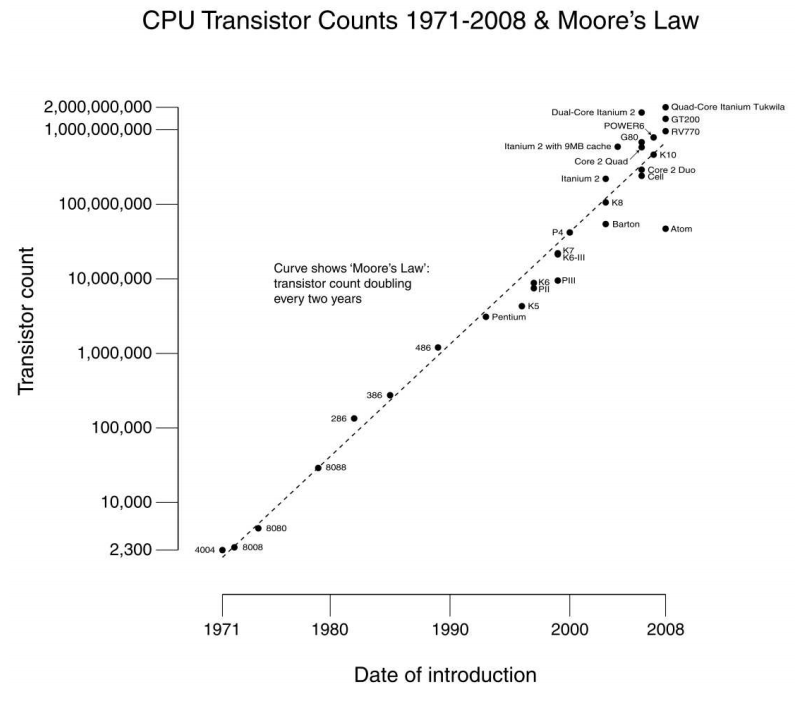
\includegraphics[scale=0.5]{figures/moores-law.png}
	\caption{Curve showing Moore's Law transistor count doubling every two years}
	\label{fig:moores-law}
\end{figure}

\section{Parallel Computing}

\subsection{Flynn's Classifications}

Flynn's classifications refers to a classigiction for computers based on their instruction and data streams. Table \ref{tab:flynn} shows these classifications. A more detailed description is given below:
\begin{itemize}
	\item \textbf{SISD (Single Instruction, Single Data)} -- in a single processor computer, a single stream of instructions is generated, which operate on a single stream of data
	\item \textbf{MIMD (Multiple Instruction, Multiple Data)} -- general-purpose multiprocessor system. Each processor has a separate program with its own instruction stream, with each stream operating on their own stream of data. 
	\item \textbf{SIMD (Single Instruction, Multiple Data)} -- specifically designed computer system where this are multiple computer programs with the \textbf{smae} instruction stream. Each program operates on different data however, meaning data can be operated on \textbf{massively in parallel} (e.g. GPUs, Map/Reduce).
	\item \textbf{MISD (Multiple Instruction, Single Data)} -- Single data items are piped through a \textit{sequence} of processors. By having the same instruction performance on the same data more than once, it is possible to have a fault tolerance mechanism based on redundancy (for example, if one processor crashes during the instruction, another processor would've performed the instruction).
\end{itemize}

\begin{table}
	\centering
	\begin{tabular}{|l|l|l|}
		\hline
		& \textbf{Single Instruction} & \textbf{Multiple Instruction} \\
		\hline
		\textbf{Single Data} & SISD & MISD \\
		\hline
		\textbf{Multiple Data} & SIMD & MIMD \\
		\hline
	\end{tabular}
	\caption{Flynn's classifications on computer streams}
	\label{tab:flynn}	
\end{table}

For multiple processors, the \textbf{Multiple Program - Multiple Data} structure can be used, in which each processor executes its own program. An alternative to this is \textbf{Single Program - Multiple Data (SPDM)}, where each processor executes its own copy of a single source program (said programs do have to be synchronised though).

Throughout this document and in MPI, a similar structure to SPDM is used. Each processor has the same program (same code), but the \textit{behaviour} of each process can actually be specified in code (based on process IDs for example).  With this, it is possible to write different programs for each processor. However, it is more common to use a \textbf{master-worker} structure (as shown in figure \ref{fig:master-worker}). Here, the \textbf{master} is the central control point, which farms out work to each worker process and aggregates the final results.

Note that SPDM is more appropriate for \textbf{static process creation}, where all processes start when the overall system starts and no new processes are added.

TODO: master-worker diagram

\subsection{Shared and Distributed Memory}

Traditionally, a process executes a program stored in memory. Each main memory location has an address represented in $b$ bits, whose value starts at 0 and can extend $2^b - 1$. Figure \ref{fig:single-process-memory} illustrates a single process with its own private space of memory.

TODO: single process memory figure

There are two principal types of parallel systems. Systems with \textbf{shared memory}, where all processes share (read/write) to the same block of memory) and systems with \textbf{distributed memory}, where each process has its own private memory store and cannot directly access the other process' memory. Hybrids of the two types are possible, such as distributed-shared memory, which MPI uses. Figures \ref{fig:multi-process-shared-memory}, \ref{fig:multi-process-distributed-memory} and \ref{fig:multi-process-hybrid-memory}  show the shared, distributed and hybrid architectures respectively.

TODO: shared memory diagram
TODO: distributed memory diagram
TODO: annotated distributed-shared memory diagrams (with my notes on the slides).

There are potential issues with shared memory programming. Because each process is reading/writing to the resources, \textbf{race conditions} can occur. These are hard to find and mean that the results of your system may differ from run to run. To prevent these, you need to identify areas which cause different output if the order of processes accessing it is different, called \textbf{critical sections}, and use locks (e.g. mutual exclusion) to prevent a processing writing to data another process is reading.

However, even when using locks to prevent race conditions, other problems can occur. An example of this is \textbf{deadlock}. The deadlock problem is when a set of blocked processes are each holding a resource and waiting to acquire a resource held by another process in the set. For example, a system has two disk drives. $P_1$ and $P_2$ each hold one disk drive and each needs the other one to continue. However, since the processes are constantly waiting for the other resource before releasing theirs, both processes are in a state of deadlock.

These problems can be avoided by using \textbf{distributed memory}. Since each process has its own local memory, which only it can access, race conditions cannot occur. This means that if a process wants to operate on some data, that data must be stored in its local memory. What happens if process A wants to operate on data owned by another process B? Then those two process must \textbf{communicate}, with process B sending the required data to process A. 

The mechanism which allows process to communicate like that is called\textbf{message passing}, and its the only way two processes can communicate. Note that this communication is typically performed over a network, which means communication can have a lot of overhead.  A good parallel system tries to minimise the communication required.

\paragraph{\textbf{NOTE:}} Distributed memory is used throughout the rest of this document.

\paragraph{}

Each process could be connected to \textbf{every other process} in the system, but this becomes very complicated, introduces difficult bugs and means there is $n^2$ communications overhead. Common process communication architectures are shown in Figure \ref{fig:common-process-architecutres}.

TODO: have a diagram with grid, hypercube and tree which are clearly labelled and has my notes on
	
\subsection{Parallel Performance Theory}

\subsection{Execution Time Analysis}
\label{sec:exec-time-analysis}

Throughout parallel performance analysis, the following variables are typically used:
\begin{itemize}
	\item $p= $ number of processes
	\item $n= $ number of data items (problem size)
	\item $t_s= $ sequential execution time
	\item $t_p= $ parallel execution time
\end{itemize}

First, we need a way of deriving formulae which describe the execution time of serial and parallel problems (and how these times change as the problem size or number of processes changes).

$t_s$ is simply the number of operations performed by the algorithm, relative to the problem size $n$. $t_p$ introduces \textit{communication}, as well as computation, so it becomes a little more complicated to assess its execution time.

\begin{equation}
	t_p = t_{comm} + t_{comp}
	\label{eq:parallel-exec-time}
\end{equation}

Equation \ref{eq:parallel-exec-time} gives a formula for parallel execution time, where $t_{comm}$ is the overall time processes spend communicating between each other and $t_{comp}$ is the overall time spent computing. For the theoretical analysis, it is assumed all processes \textbf{operate at the same speed}.

$t_{comp}$ typically depends on $n$ and $p$. When analysing computation time, always use the worst case (similar to time complexity), by analysing the most complex process. 

$t_{comm}$ depends on the number of messages passed and the size of each message. It also depends on the interconnection structure of the processes and the mode of transfer (e.g. network connection, piped file, etc.). Equation \ref{eq:time-comm-formula} gives a formula for communication time for a single message, where $t_{startup}$ is a constant that represents \textbf{message latency} (overhead), $t_{data}$ is a constant that represents the transmission time for a single data item and $m$ is the number of data items sent in the message.

\begin{equation}
	t_{comm} = t_{startup} + m t_{data}
	\label{eq:time-comm-formula}
\end{equation}

\paragraph{\textbf{NOTE:}} The computation/communication ratio $\frac{t_{comp}}{t_{comm}}$ can be used as a metric to assess the scalability of an implementation.

\paragraph{\textbf{EXAMPLE ALGORITHM}} Consider summing an array of $n$ numbers using $p$ processors. Suppose the numbers are evently distributed across the processes, including the master process. This means $n$ is divisible by $p$ (which is a reasonable approximation for large $n$. After summing all the sub-arrays, the master process adds the partial sub-array sums to get the final answer.

\paragraph{\textbf{ANALYSIS}} Each process, including the master, adds its $\frac{n}{p}$ numbers concurrently with the other processes. This means each processor performs ($\frac{n}{p} - 1$) additions. Let $t_{comp1} = (\frac{n}{p} - 1)$ be the running time for this.

The master process receives its partial sums back from all of the other processes, making $t_comm = (p - 1)(t_{startup} + t_{data})$. 

Finally, the master adds all the partial sums, which takes $t_{comp2} = p - 1$ operations.

Therefore, $t_{comp} = t_{comp1} + t_{comp2} = (\frac{n}{p} - 1) + p - 1 = \frac{n}{p} + p - 2$ and $t_comm = (p - 1)(t_{startup} + t_{data})$. With a serial algorithm, $n - 1$ additions are performed to sum all $n$ numbers up. This makes the overall computations times:
\begin{multline}\\
	t_s = n - 1 \\
	t_p = t_{comm} + t_{comp} = (p - 1)(t_{startup} + t_{data}) + \frac{n}{p} + p - 2 \\
\end{multline}

\subsubsection{Speedup}

Speedup measures how much parallelising a problem across $p$ processors speeds up the computation time. It is defined as:
\begin{equation}
	S(p) = \frac{t_s}{t_p}
	\label{eq:speedup}
\end{equation}
Ideally, speedup is linear in terms of $p$, meaning that you get a linear increase in speedup as you increase the number of processes used for the problem. However, \textbf{Amdahl's Law} states that:
\begin{equation}
	S(p) \leq \frac{p}{1 + (p - 1)f}
	\label{eq:amdahl-law}
\end{equation}
where $f$ is a \textbf{fraction} of the program that is \textbf{inherently serial} (there is no way to parallelise it), relative to \textit{serial} execution time. Figure \ref{fig:amdahl} shows that the increase in speedup is reduced as you increase the process count after a certain point (based on the fraction of the program which is serial). This implies there is a little point on using \textit{large} numbers of processors. For example, Figure \ref{fig:amdahl} shows that increasing the number of processors from 16 to 32 when $f = 0.2$ has almost no affect no speedup.

\begin{figure}
	\centering
	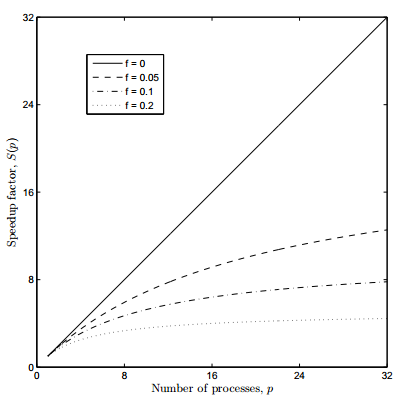
\includegraphics[scale=0.7]{figures/amdahl-law.png}
	\caption{Amdahl's Law}
	\label{fig:amdahl}
\end{figure}

The speedup of the number summing algorithm from section \ref{sec:exec-time-analysis} is:
\begin{equation}
	S(p) = \frac{t_s}{t_p} = \frac{n - 1}{(p - 1)(t_{startup} + t_{data}) + \frac{n}{p} + p - 2}
\end{equation}

\subsubsection{Efficiency}

Amdahl's law is based on the assumption that a problem has a \textbf{fixed size}, implying that $t_s$ is fixed. This is rarely the case. \textbf{Gustafson's Law} argues that is more relevant to make the parallel execution time $t_p$ fixed. Therefore,as the number of processors is increased, the problem size is increased at a rate which maintains the \textbf{same parallel execution time} (does not become slower, i.e. $t_p$ is not higher). This is done to assess the \textbf{scalability} of a parallel implementation.

Gustafson's Law is given by Equation \ref{eq:guastafson-law}, where $f$ is now the fraction of the program which is serial relative to \textit{parallel} execution time (opposite of Amdahl's law!)
\begin{equation}
	S(p) \leq f + (1 - f)p
	\label{eq:guastafson-law}
\end{equation}

\begin{figure}
	\centering
	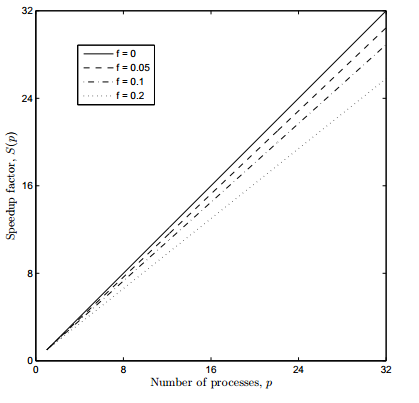
\includegraphics[scale=0.7]{figures/gustafson-law.png}
	\caption{Gustafson's Law}
	\label{fig:gustafson}
\end{figure}

This results in a measure of \textbf{efficiency}, instead of speedup. This measurement takes into consideration extra overhead introdeuced by parallelising the problem (e.g. from message passing, excess computation, idle time and so on). Equation \ref{eq:efficiency} gives the formula to compute efficiency.

\begin{equation}
	E(p) = \frac{(\frac{t_s}{t_p})}{p} = \frac{S(p)}{p}
	\label{eq:efficiency}
\end{equation}

The efficiency of the number summing algorithm from section \ref{sec:exec-time-analysis} is:
\begin{equation}
	E(p) = \frac{t_s}{pt_p} = \frac{n - 1}{p(p - 1)(t_{startup} + t_{data}) + n + p^2 - 2p}
\end{equation}

\paragraph{\textbf{NOTE:}} \textbf{Divide and conquer} is one way of partitioning a problem up which typically improves scalability. This is because the tree structure resulting from breaking the problem into subproblems recursively provides \textbf{logarithmic} time complexity. Figure \ref{fig:summing-numbers-speedup} shows the differing speedup factors of using a flat decomposition of the problem (1a, the example from this document) with a tree-based decomposition (1b). 1a's speedup speedup decreases in $p^2$ whereas 1b decreases in $plog_8$. Lower complexities when discussing change in speedup mean better parallel algorithms.

\begin{figure}
	\centering
	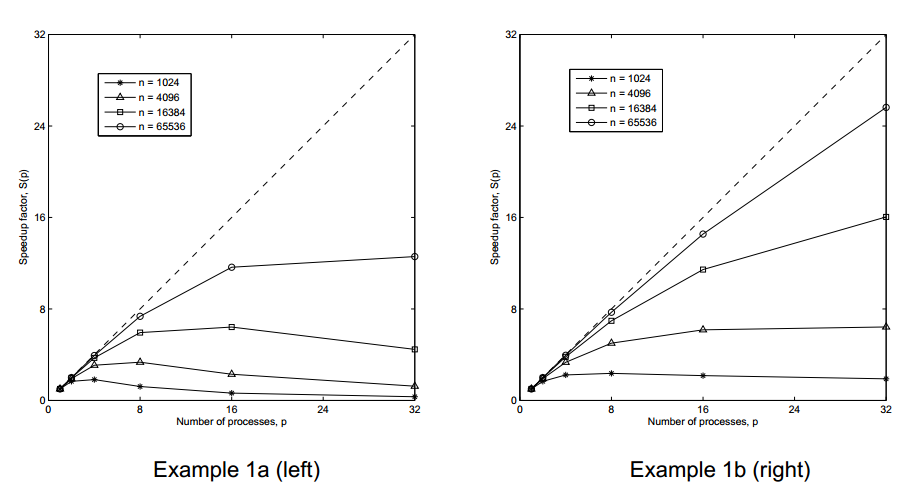
\includegraphics[scale=0.5]{figures/summing-numbers-speedup-plots.png}
	\caption{Speedup against processes for varying problem sizes for two parallel implementations of \textbf{summing numbers}}
	\label{fig:summing-numbers-speedup}
\end{figure}

\subsubsection{Scalability and Iso-efficiency}

\textbf{Strong scalability} relates to the way the execution time scales with the number of processes $p$ for a fixed problem size $n$. \textbf{Weak scalability} is similar, but is concerned how execution time scales with a fixed problem size \textbf{per processor}. These involve varying values for $p$ but a fixed $n$.

\textbf{Isoefficiency} describes the relationship between the problem size $n$ and the number of processors $p$, if the relationship maintains \textbf{constant, non-zero, efficiency} asymptotically as $n,p \rightarrow \infty$. The idea value for this constant is 1, as you have maximum scalability. Isoefficiency provides a commonly-used indicator of the scalability of a parallel algorithm. The more slowly $n$ increases with $p$, the better.

This relation can be extracted from the efficiency expression $E(p)$ and is described in the form $n \propto p$.
\begin{itemize}
	\item Divide through highest power of $n$ on the numerator of $E(p)$ ($t_s$) to get a non-zero constant on the numerator. It's okay if it's just \textit{close} to one, so if it's a fraction with $n$ as the denominator, then it's \textit{essentially} constant for large $n$ (tends to 1).
	\item Use the power of $n$ used for the division as $n$ in the isoefficiency description
	\item Look at the resultant denominator and use the highest power of $p$ as $p$ in the isoefficiency
\end{itemize}
That is, isoefficiency is $n^{a} \propto p^{b}$, where $a$ and $b$ are the highest power of $n$ in the numerator and highest power of $p$ in the denominator respectively.

Using the number summing algorithm from Section \ref{sec:exec-time-analysis}, we derive the isoefficiency like so:
\begin{equation}
	E(p) = \frac{t_s}{pt_p} = \frac{n - 1}{p(p - 1)(t_{startup} + t_{data}) + n + p^2 - 2p}
\end{equation}
Divide the entire equation by a factor of $n$ (highest power of $n$) such that the numerator of $E(p)$ is constant or less. That is, divide $E(p)$ by $n$:
\begin{equation}
	E(p) = \frac{t_s}{pt_p} = \frac{\frac{n - 1}{n}}{\frac{p(p - 1)(t_{startup} + t_{data}) + n + p^2 - 2p}{n}} = \frac{1 - \frac{1}{n}}{\frac{(p^2 - p)}{n}(t_{startup} + t_{data}) + 1 + \frac{p^2}{n} - \frac{2p}{n} }
\end{equation}
We have an \textit{almost} constant numerator by dividing $E(p)$ by $n$, and the highest power on the denominator is $p^2$. Therefore, the number summing algorithm has an isoefficiency of $n \propto n^2$.

\paragraph{\textbf{ISOEFFICIENCY OF JACOBI ITERATION}} The serial and parallel execution times of parallel Jacobi iteration are:
\begin{multline}\\
	t_s = 2n^2 \\
	t_p = \frac{2n^2}{p} + 2(p - 1)(t_{startup} + \frac{n}{p}t_{data}) = \frac{2n^2}{p} + 2(p - 1)(t_{startup}) + 2(p - 1)(\frac{n}{p}t_{data})
\end{multline}
Simplifying $t_p$ by multiplying it $p$ results in:
\begin{equation}
	pt_p = 2n^2 + 2p(p - 1)(t_{startup}) + 2p(p - 1)(\frac{n}{p}t_{data}) \\
	=  2n^2 + 2p(p - 1)(t_{startup}) + 2n(p - 1)t_{data}
\end{equation}
Meaning the efficiency is:
\begin{multline} \\
E = \frac{2n^2}{2n^2 + 2p(p - 1)(t_{startup}) + 2n(p - 1)t_{data}} \\
\end{multline}
Dividing by highest power of $n$ in numerator gives:
\begin{multline} \\
	E = \frac{2}{2 + (\frac{2p^2}{n^2} - \frac{2p}{n^2})t_{startup} + (\frac{2p}{n} - \frac{2}{n})t_{data}} \\
\end{multline}
The highest power of $p$ in the numerator is $p^2$, meaning $n^2 \propto p^2 \implies n \propto p$. Therefore, Jacobi iteration has an isoefficiency of $n \propto p$.

TODO: look at parallel worksheet

\subsection{Pipelining for Sequential Tasks}

\textbf{Pipelining} is a technique for parallelising tasks that have a \textbf{sequential} element to them. Examples of problems where pipelining may be useful include:
\begin{itemize}
	\item forward elimination to turn matrix into echelon form
	\item solving triangular systems using back substitution (Gaussian Elimination)
\end{itemize}

\subsection{Parallelising Heat Diffusion Problem}
\label{sec:heat-diffusion-parallel}

This section discusses different ways to parallelise a solver for the heat diffusion problem discussed in Section \ref{sec:bvp}. Since the system of equations for the problem is sparse has a tri-diagonal structure, the Jacobi iteration of node $(i, j)$ can be derived like so:
\begin{equation}
	u_{i,j}^{(k + 1)} = \frac{1}{4}\left( u_{i-1,j}^{(k)} + u_{i,j-1}^{(k)} + u_{i+1,j}^{(k)} + u_{i,j+1}^{(k)} - h^2f(\vec{x}_{i,j}) \right)
	\label{eq:heat-diffusion-jacobi}
\end{equation}
It is also possible to use Gauss-Seidel in the standard way:
\begin{equation}
	u_{i,j}^{(k + 1)} = \frac{1}{4}\left( u_{i-1,j}^{(k+1)} + u_{i,j-1}^{(k+1)} + u_{i+1,j}^{(k)} + u_{i,j+1}^{(k)} - h^2f(\vec{x}_{i,j}) \right)
	\label{eq:heat-diffusion-lex-gauss}
\end{equation}

The form of Gauss-Seidel used in Equation \ref{eq:heat-diffusion-lex-gauss} is known as \textbf{lexicographic Gauss-Seidel}. To compute the latest value for node at $(i, j)$, we use the latest values of nodes $(i - 1, j)$ and $(i, j - 1)$ and the old values (from the previous iteration $k$) of nodes $(i + 1, j)$, $(i, j + 1)$. This is because the latest values for the latter two nodes has not been computed yet.

TODO: figure illustrating lexicograpghic Gauss-Seidel

TODO: figure illustrating red-black Gauss-Seidel

One problem when using lexicographic ordering for Gauss-Seidel is that as you increase the number of processes, you increase the number of iterations required to converge to a solution. This is because the \textit{boundary} values each process contains depend on newly computed values from other processes. Since those new values (used for Gauss-Seidel iteration) are not received by a process until \textit{after} the whole iteration, the current iteration uses old values where new values should have been used, which slows the convergence.

\textbf{Red-black Gauss-Seidel} eliminates this problem. It takes the same number of iterations as Gauss-Seidel to converge on a single processor, but the number iterations does not increase as you add more processes like lexicographic. This overall makes the red-black ordering \textbf{more scalable} than the lexicographic ordering

Each of the nodes in the regular mesh are coloured red or black in an alternating fashion, so all the neighbours of a red node are black and vice versa. This is illustrated in Figure \ref{fig:redblack-ordernig}. Iteration $(k + 1)$ works as follows:
\begin{enumerate}
	\item Send/receive black nodes to/from neighbouring processes (values from iteration $(k)$)
	\item Update red nodes by computing their values for $k + 1$
	\item Send/receive red nodes to/from neighbouring processes (values from iteration $(k + 1)$)
	\item Update black nodes by computing their values for $k + 1$
\end{enumerate}
Now there are two lots of communication for each iteration and two stages of computation per iteration. Equation \ref{eq:heat-diffusion-redblack-gauss} shows the formulae used to update red and black.

\begin{multline}\\
	\mathbf{RED\;NODES}: \;\;\;\;\;
	u_{i,j}^{(k + 1)} = \frac{1}{4}\left( u_{i-1,j}^{(k)} + u_{i,j-1}^{(k)} + u_{i+1,j}^{(k)} + u_{i,j+1}^{(k)} - h^2f(\vec{x}_{i,j}) \right) \\
	\mathbf{BLACK\;NODES}: \;\;\;\;\;
	u_{i,j}^{(k + 1)} = \frac{1}{4}\left( u_{i-1,j}^{(k+1)} + u_{i,j-1}^{(k+1)} + u_{i+1,j}^{(k+1)} + u_{i,j+1}^{(k+1)} - h^2f(\vec{x}_{i,j}) \right) \\
	\label{eq:heat-diffusion-redblack-gauss}
\end{multline}

\subsection{Partitioning Strategies}

This section describes common strategies for partitioning a problem into work that can be solved by multiple parallel processes. The heat diffusion problem in Section \ref{sec:bvp} will be used an example to illustrate how these partitioning strategies work, as it is common to want to solve systems of equations with sparse structures.

\subsubsection{Row/Strip Decomposition}

Strip, or row, decomposition allocates \textbf{one or more contiguous rows} to each process sequentially. the allocation should try and be as even as possible so each process has roughly the same number of rows. For example, if there are 10 rows in a matrix and 5 processes, then each process is given a strip of two rows (process 1 getting rows 1 and 2, process 2 getting rows 3 and 4, etc.). This means each process gets a strip of $\frac{N - 1}{p}$ rows, where $N$ is the problem size and $p$ is the number of processors.

With the heat diffusion problem, an equation for a node depends on the values of all adjacent nodes. So how does a process receive a value for a node adjacent to one on the \textbf{process boundary}? That is, how does it get the updated value of a node that is handled by another process? This is done through communication -- each process communicates with the \textbf{previous and next} processes that deal with the rows directly above and below the rows the current process deals with. A process sends the values of nodes at its boundary and receives the values of nodes on the previous/next processes' boundaries. Figure \ref{fig:heat-diffusion-strip-decomposition} illustrates the strip allocation and how processes communicate at the boundaries.

One issue with this is when the number of rows (problem size) is not divisible by the number of processors, the number of rows to allocate to a process is \textit{fractional}. This is handled by computing the remainder of $\frac{N - 1}{p}$, $r = (N - 1) \mod p$. Due to the nature of the remainder, $r < p$. Therefore, simply compute the remainder and allocate $\frac{N - 1 - r}{p}$ rows to each process, giving \textbf{one extra row} to the first $r$ processes.

We can analyse the speed-up and efficiency of this problem using row/strip decomposition. Let $n = N -1$. Suppose Jacobi iteration is used to solve the system ($O(n^2)$). A serial implementation takes 4 Jacobi iterations, which makes $t_s = 4n^2$.

Each process needs to communicate with its \textbf{two boundary processes}, sending its boundary values and receiving the boundary values from the other process. This results in four messages, where each message sends a row of $n$ values. Therefore, $t_{comm} = 4(t_{startup} + nt_{data})$.

$t_{comp} = \frac{4n^2}{p}$, since the same amount of work is performed as the serial implementation overall, it is just distributed across $p$ processes. This makes $t_p = t_{comp}  + t_{comm} = \frac{4n^2}{p} + 4(t_{startup} + nt_{data})$. Speed and efficiency are given in Equation \ref{eq:row-decomp-heat-speedup-efficiency}.

\begin{multline} \\
	S(p) = \frac{t_s}{t_p} = \frac{4n^2}{\frac{4n^2}{p} + 4(t_{startup} + nt_{data})} \\
	E(p) = \frac{t_s}{popt_p} = \frac{4n^2}{4n^2 + 4p(t_{startup} + nt_{data})}
	\\
	\label {eq:row-decomp-heat-speedup-efficiency}
\end{multline}
To find the isoefficiency, we can divide $E(p)$ by the highest power on the numerator. Dividing $E(p)$ by $4n^2$ gives us:
\begin{equation}
	E(p) = \frac{1}{1 + \frac{p}{n^2}(t_{startup} + t_{data}} = \frac{1}{1 + \frac{p}{n^2}t_{startup} + \frac{p}{n}t_{data}}
	\label {eq:row-decomp-heat-isoefficiency}	
\end{equation}
So the isoefficiency of heat diffusion with row decomposition is $n \propto p$. It is \textbf{not} $n^2 \propto p$ because $\frac{p}{n}$ in the denominator is actually the highest value for $p$, since $\frac{p}{n^2}$ would result in a smaller number.

\begin{figure}
	\centering
	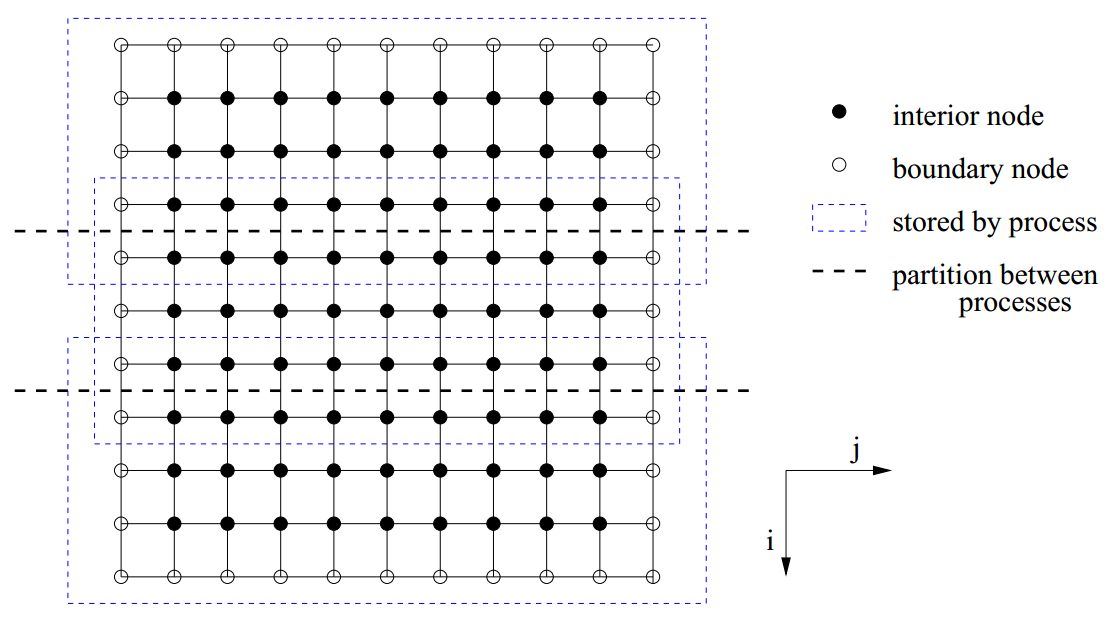
\includegraphics[scale=0.4]{figures/strip-decomposition.png}
	\caption{Strip partition of an $11 \times 11$ mesh ($N = 10$) across 3 processes}
	\label{fig:strip-decomposition}
\end{figure}

\subsubsection{Block Decomposition}

Instead of splitting the system of equations/mesh in strips of rows for the heat diffusion problem, the system could be split into blocks. \textbf{Block decomposition} partitions the 2D mesh into sub-meshes, where each sub-mesh is a uniform square. Figure \ref{fig:block-decomposition} illustrates how the heat diffusion mesh can be separated into blocks. As before, let $n = N - 1$ and $n^2$ be the size of the square mesh.

\paragraph{\textbf{NOTE:}} Typically, each block is a $\frac{n}{\sqrt{p}} \times \frac{n}{\sqrt{p}}$ sub-mesh/matrix, which means that the problem size used ($n$) must be divisible by $\sqrt{p}$.
\paragraph{}

Here, each process has at most \textbf{four boundaries}, which means it needs to communicate with four processes. Like strip decomposition, each process needs to send and receive the updated boundary values to each of its neighbouring processes, which results in a total of 8 messages per process per iteration. Each message send/receives one side of the block, which has  $\frac{n}{\sqrt{p}}$ elements. This makes $t_{comm} = 8 \left( t_{startup} + \frac{n}{\sqrt{p}}t_{data} \right)$.

Each block has $\frac{n}{\sqrt{p}} \times \frac{n}{\sqrt{p}} = \frac{n}{p}$ elements. Therefore, the total number of work is evenly distributed across all $p$ processes. Since $t_s = 4n^2$, this makes $t_{comp} = \frac{4n^2}{p}$.

$t_p = t_{comp} + t_{comm} = \frac{4n^2}{p} + 8 \left( t_{startup} + \frac{n}{\sqrt{p}}t_{data} \right)$, which makes the speed and efficiency:
\begin{multline} \\
	S(p) = \frac{t_s}{t_p} = \frac{4n^2}{\frac{4n^2}{p} + 8 \left( t_{startup} + \frac{n}{\sqrt{p}}t_{data} \right)} \\
	E(p) = \frac{t_s}{pt_p} =
	\frac{4n^2}{p \left( \frac{4n^2}{p} + 8 \left( t_{startup} + \frac{n}{\sqrt{p}}t_{data} \right) \right) } =
	\frac{4n^2}{4n^2 + 8p\left( t_{startup} + \frac{n}{\sqrt{p}}t_{data} \right)} =
	\frac{4n^2}{4n^2 + 8pt_{startup} + 8p\frac{n}{\sqrt{p}}t_{data}}
	\\
	\label {eq:block-decomp-heat-speedup-efficiency}
\end{multline}
Dividing $E(p)$ by $n^2$ to get numerator constant (highest power of $n$), we get:
\begin{equation}
	\frac{E(p)}{n^2} = \frac{4}{4 + \frac{8p}{n^2}t_{startup} + \frac{8\sqrt{p}}{n}t_{data}}
	\label {eq:block-decomp-heat-isoefficiency}
\end{equation}
Since $\frac{8\sqrt{p}}{n}$ is present in the denominator, the isoefficiency is $n \propto \sqrt{p}$.

This means block decomposition has different iso-efficiency, hence different scalability, than strip decomposition. Figure \ref{fig:row-block-heat-diffusion-speedup} shows the speedup factor of the heat diffusion problem when using strip and block decomposition. Notice how theoretically, block decomposition has greater scalability than row decomposition, because the speedup increases much more as the number of processes increases.

\begin{figure}
	\centering
	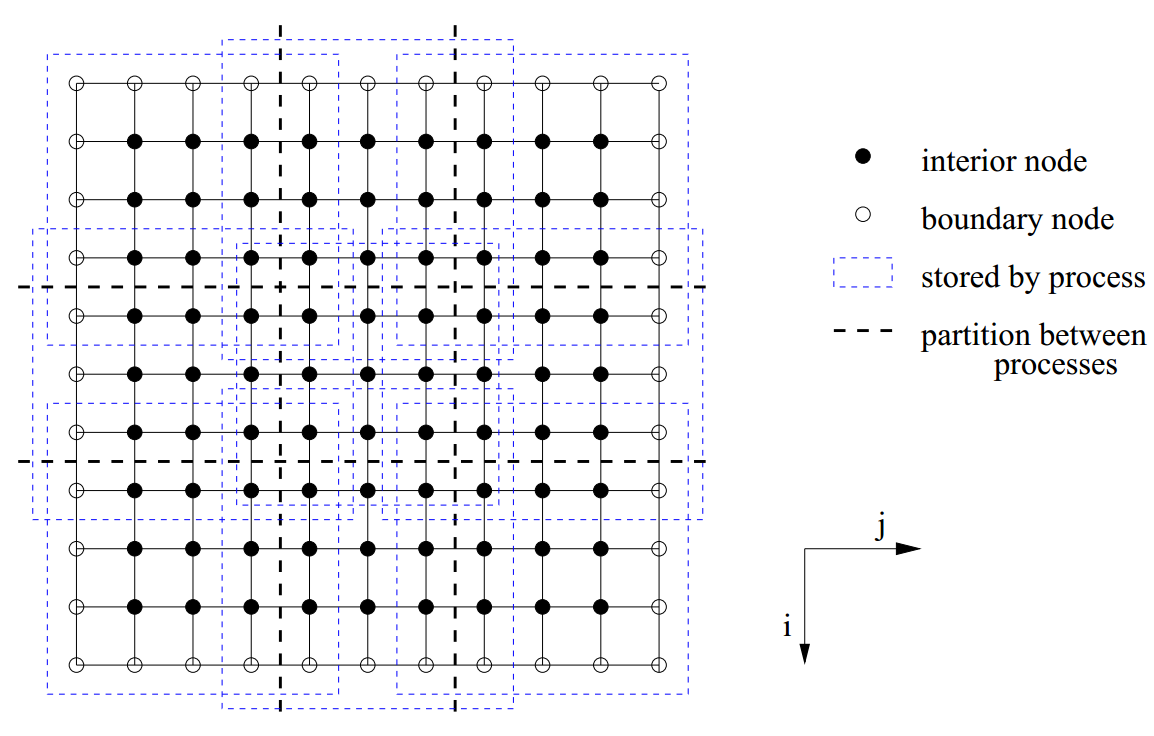
\includegraphics[scale=0.4]{figures/block-decomposition.png}
	\caption{Block partition of an $11 \times 11$ mesh ($N = 10$) across 9 processes}
	\label{fig:block-decomposition}
\end{figure}

\begin{figure}
	\centering
	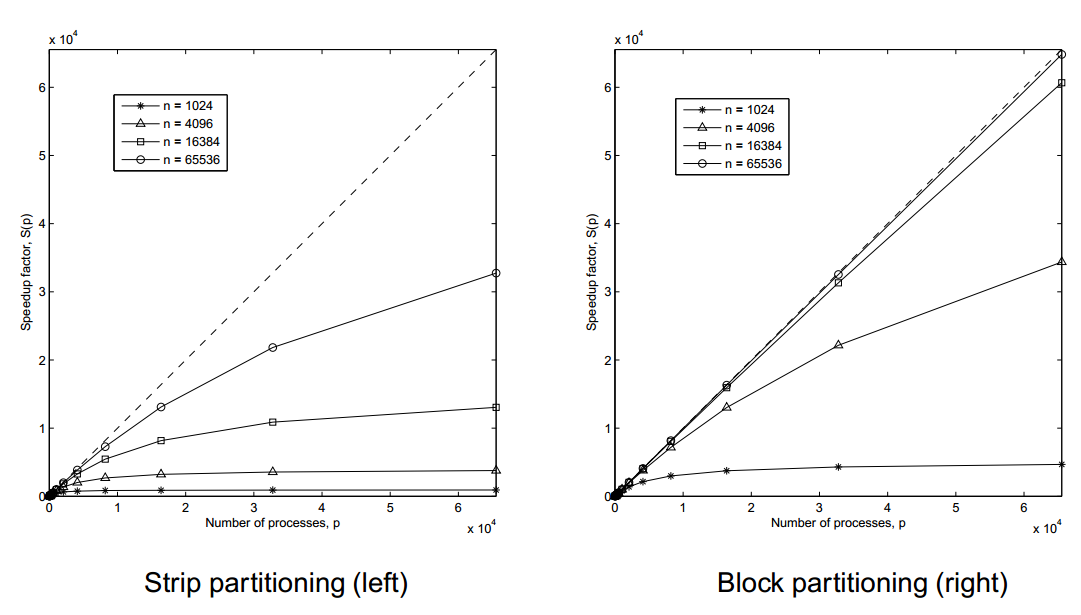
\includegraphics[scale=0.6]{figures/strip-block-speedup.png}
	\caption{Speedup factors of strip and block decomposition for varying problem sizes of the heat diffusion problem}
	\label{fig:row-block-heat-diffusion-speedup}
\end{figure}

\section{Scientific Computing}

\subsection{Common Linear Algebra and How To Partition Them}

\begin{table}[H]
	\centering
	\begin{tabular}{|p{5cm}|p{2cm}|p{9cm}|}
	\hline
	\textbf{Operation} & \textbf{Complexity} & \textbf{Partitioning Strategy} \\
	\hline
	\textbf{Vector Addition} & $O(n)$ & Strip partitioning. Split the vector into $\frac{n}{p}$ chunks and send off to $p$ processes\\	
	\textbf{Vector Dot/Scalar Product} & $O(n)$ & Strip partitioning. Split the vector into $\frac{n}{p}$ chunks and send off to $p$ processes\\	
	\textbf{Matrix Addition} & $O(n^2)$ & Block partitioning. Split matrix into $\frac{n}{p}$ sub-matrices and send off to $p$ processes \\
	\textbf{Matrix Multiplication} & $O(n^3)$ & Block partitioning. Split $n \times n$ matrix into $s^2$ $(\frac{n}{s} \times \frac{n}{s})$ sub-matrices and send off to $p$ processes. Note that $\sqrt{p}$ should be an integer. \\
	\textbf{Gaussian Elimination (Forward Elimination Step)} & $O(n^2)$ &  Pipelining of processes could be used in a similar way as the back substitution, with cyclic decomposition used to distributed work more evenly, since the bottom rows are more work than the top (opposite of back substitution). \\
	\textbf{Gaussian Elimination (Back Substitution Step)} & $O(n^3)$ &  Use pipelining, going from bottom row to top. Each process deals with a \textbf{contiguous} block of rows and passes the computed coefficients to the next process, as a chain process. \textbf{Cyclic decomposition} may be useful here, since cycling through processes when allocating rows means that the work is distributed more evenly than block (rows at top of matrix have much more work than rows at the bottom, since an upper triangular matrix is being solved). \\
	\hline
	\end{tabular}
	\caption{Complexity and partitioning strategies for different linear algebra operations ($n= $problem size and $p= $ number of processors)}
\end{table}

\subsection{Solving Systems of Equations}

\subsubsection{What are Systems of Equations?}

A system of equations is a set of $n$ \textbf{linear} equations for $n$ unknown values $x_0$, $x_1$, ..., $x_{n-1}$. This looks like:
\begin{multline}\\
	a_{00}x_0 + a_{01}x_1 + a_{02}x_2 + ... + a_{0n -1}x_{n - 1} = b_0 \\
	a_{10}x_0 + a_{11}x_1 + a_{12}x_2 + ... + a_{1n -1}x_{n - 1} = b_1 \\
	\vdots \\
	a_{i0}x_0 + a_{i1}x_1 + a_{i2}x_2 + ... + a_{in -1}x_{n - 1} = b_i \\
	\vdots \\
	a_{n-10}x_0 + a_{n-1n1}x_1 + a_{n2}x_2 + ... + a_{n-1n -1}x_{n - 1} = b_{n-1} \\
	\label{eq:system-of-equations}
\end{multline}

\subsubsection{Gaussian Elimination (Direct Method)}

\textbf{Gaussian elimination} is a direct method for solving systems of equations, which means it is \textbf{guaranteed} to find the exact solution after enough time. However, it is an $O(n^3)$ algorithm, which makes it very slow for large matrices -- the amount of work is fixed but can be very large.

Additionally, the effect of \textbf{rounding error} means that the result may not be accurate, since the computed numbers may be drifting away from the exact solution as more and more operations on the matrix is performed. Finite precision arithmetic means that Gaussian Elimination will not \textit{always} product a perfect result.

\subsubsection{Iterative Methods}

An alternative to direct methods are iterative methods. Instead of trying to find the exact solution, these attempt to find a "good enough" approximation of the solution. Iterative methods improve an approximation $\vec{x}^{k}$ to the solution of $Ax = b$, with each iteration taking the form $\vec{x}^{k + 1} = f(\vec{x}^{k})$. These methods require an initial iterate (guess), $\vec{x}^{0}$. A reasonable approximation to $x$ is typically available through simpler means, so that is used as the initial iterate.

\paragraph{\textbf{NOTE:}} If a system has 100000 or more unknowns, iterative algorithms are almost certainly used, as $O(n^3)$ direct methods are just too expensive computationally.

\paragraph{}

TODO: advantages of iteration methods over direct method (look at notes). also summarise advantages of jacboi, gauss ansd SOR

With iterative methods, the following questions are raised:
\begin{itemize}
	\item when does the iteration converge to a solution? Do they always converge to a solution or is there a chance the algorithm could iterate forever?
	\item when it does converge, how quickly can it do so?
	\item when is the approximation accurate enough? When do we decide to stop iterating? (\textbf{stopping criteria})
	\item when is it faster than a direct approach? (if it requires less than $n$ iterations)
\end{itemize}

\subsubsection{Jacobi Iteration}

Jacobi iteration takes the form of:
\begin{multline}
	\mathbf{x}^{k+1} = \mathbf{x}^{k} + \mathbf{D}^{-1}(\mathbf{b} - \mathbf{Ax}^{k})\\
	\label{eq:jacobi}
\end{multline}
Computationally, the iteration is often performed element-by-element. Each element $i \in \lbrace 0, 1, ..., n - 1 \rbrace$ is updated like so:
\begin{multline}
	x_i^{(k+1)} = x_i^{(k)} + \frac{1}{a_{ii}}(b_i - \sum_{j=0}^{n - 1} {a_{ij}x_{j}^{(k)}})
	\\
	\label{eq:jacobi-elembyelem}
\end{multline}

The cost of a single iteration of the algorithm is $O(n^2)$ ($O(n)$ for a sparse system). If it takes $\geq n$ iterations to find a good approximation of the solution, then it may worth using a direct method instead, as the complexity if $O(n^3)$ anyway. Commonly used stopping criteria for Jacobi iteration are listed in Section \ref{sec:stopping-criteria}.

To perform Jacobi iteration in parallel, different chunks of elements could be sent off to each process. Each process needs the entire system in order to perform a Jacobi iteration on its elements.

There isn't a substantial difference between block and cyclic decomposition for Jacobi iteration. Due to block decomposition result in sending/receiving/processing of \textbf{contiguous memory} blocks, it is often preferred.

\subsubsection{Gauss-Seidel Iteration}

Gauss-Seidel iteration builds upon Jacobi. Instead of using all the values from iteration $k$ to compute iteration $k+1$, it uses values from $k+1$ it has already computed in the current iteration.

\begin{multline}
	x_i^{(k+1)} = x_i^{(k)} + \frac{1}{a_{ii}}(b_i - \sum_{j=0}^{i - 1} {a_{ij}x_{j}^{(k+1)}} - \sum_{j=i+1}^{n - 1} {a_{ij}x_{j}^{(k)}})
	\\
	\label{eq:gauss-seidel-elembyelem}
\end{multline}

Due to the nature of the formula and how some elements require values computed from the current iteration (which may have been computed on another process), each iteration is no longer \textbf{embarrassingly parallel}. However, we are free to choose the \textit{order} in which the elements are updated, which can help simplify a parallel implementation.

\subsubsection{Successive Over-Relaxation}

TODO: serial and parallel (same as Gauss-Seidel)

\subsubsection{Iteration Stopping Criteria}
\label{sec:stopping-crtieria}

Potential \textbf{stopping criteria} for Jacobi iteration is \textbf{error tolerance}. When the exact solution is not known, the "error" of the solution is measured by the difference on iteration $k$ and $k+1$. If the difference between the two is sufficiently small, then we say the algorithm has \textbf{converged} on a solution and terminate.

An "acceptable" level of error $TOL$ is specified, then one or more of the following conditions is tested:
\begin{itemize}
	\item Maximum different in elements -- $\max_{i} |x_i^{k+1} - x_i^k| < TOL$
	\item Average difference in elements -- $[\frac{1}{n} \sum_{i=0}^{n - 1} (x_i^{k + 1} - x_i^k)^2 ]^{\frac{1}{2}} < TOL$
	\item Maximum residual vector value -- $\max_{i} |b_i - \sum_{i=0}^{n - 1} { a_{ij}x_j^k } | < TOL$
\end{itemize}

\subsection{Partial Differential Equations}

\subsubsection{Derivatives and Approximating Derivatives}
The \textbf{derivative} $u'(x)$ of a function $u(x)$ is the \textbf{rate of change} of $u$ with respect to $x$. Geometrically, this could be thought of as the \textit{slope} of the line/curve at point $x$. It is defined as:
\begin{equation}
	\frac{du}{dx} = u'(x) = \lim_{\delta x \rightarrow \infty} \frac{u(x + \delta x) - u(x)}{\delta x}
	\label{eq:derivative1}
\end{equation}
where $\delta x$ is the interval between $x$ values.

$u'(x)$ is known as a \textbf{first} derivative. The derivative of $u'(x)$, $u''(x)$  is a \textbf{second} derivative. An example of a derivatives is distance, speed and acceleration. Speed is the rate of change of distance and acceleration is the rate of change of speed. Therefore, speed is a first derivative and acceleration is a second derivative.

Derivatives can be used to find "turning points" in function (e.g. maxima/minima), as shown in Figure \ref{fig:maxima-minima}). This is useful in optimisation.  Other forms of representing derivatives include:
\begin{equation}\\
	\lim_{\delta x \rightarrow \infty} \frac{u(x) - u(x - \delta x)}{\delta x}
	\label{eq:derivative2}
\end{equation}
\begin{equation}\\
	\lim_{\delta x \rightarrow \infty} \frac{u(x + \delta x) - u(x - \delta x)}{2\delta x} \\
	\label{eq:derivative3}
\end{equation}

For smooth functions, all three definitions will lead to precisely the same derivatives. However, each of them lead to a \textbf{different} way of \textbf{approximating/discretising} a derivative (each approximation has different properties).

To approximate derivatives, $\delta x$ is given a fixed value with is greater than 0, instead of taking the limit as $\delta x \rightarrow 0$. This evaluates the slope of a \textit{nearby chord}, instead of the slope exactly at $x$. 

Equations \ref{eq:derivative1-approx}, \ref{eq:derivative2-approx} and \ref{eq:derivative3-approx} are the approximations of the derivative using the represents in Equations \ref{eq:derivative1}, \ref{eq:derivative2} and \ref{eq:derivative3} respectively. The symmetric form used in  \ref{eq:derivative3-approx} is known as \textbf{central differencing}. Equations \ref{eq:derivative1-approx}  and \ref{eq:derivative2-approx}  bias the approximation to one side or the other.

\begin{equation}
	\frac{du}{dx} \approx \frac{u(x + \delta x) - u(x)}{\delta x}
	\label{eq:derivative1-approx}
\end{equation}
\begin{equation}
	\frac{du}{dx} \approx \frac{u(x - \delta x) - u(x)}{\delta x}
	\label{eq:derivative2-approx}
\end{equation}
\begin{equation}
	\frac{du}{dx} \approx \frac{u(x + \delta x) - u(x - \delta x)}{2\delta x}
	\label{eq:derivative3-approx}
\end{equation}

Which approximation is used can greatly affect the error/inaccuracy in the result. For example, the error when approximating equation $u(x) = 1 + 5x^2 - 6x^4$ with its derivative $u'(x) = 10x - 24x^3$ is $O(\delta x)$ for the one-sided difference and $O(\delta x^2)$ for the central difference. Central differences is better in this case, because $\delta x < 1$, meaning $O(\delta x^2)$ results in a lower error than $O(\delta x)$.

Unfortunately, due to finite precision arithmetic being used on computers, it is not possible to just decrease $\delta x$ more and more and expect more accuracy. At some point, the differences between the numbers will be too small to be represented in floating point numbers, rounding will happen and the error will start increasing again. This is illustrated in Figure \ref{fig:derivative-approx-error}. A \textbf{balance} is sought out between inaccuracy caused by a less precise approximation (high values for $\delta x$) and inaccuracy caused by rounding error (low values for $\delta x$).

Approximating higher derivatives (i.e. the rate of change of a rate of change) can be achieved like so:
\begin{equation}
	\frac{d^2u}{dx^2} = u''(x) = \lim_{\delta x \rightarrow \infty} \frac{u'(x + \frac{\delta x}{2}) - u'(x - \frac{\delta x}{2})}{\delta x}
	\label{eq:higher-derivative-approx}
\end{equation}
Central differences is most commonly used to approximate a second, higher derivative. It takes a fixed value for $\delta x$ and only needs to use the original function (not its first derivative. Equation \ref{eq:higher-derivative-central-approx}
\begin{equation}
	\frac{d^2u}{dx^2} = u''(x) = \lim_{\delta x \rightarrow \infty} \frac{u(x + \delta x) - 2u(x) + u(x - \delta x)}{\delta x^2}
	\label{eq:higher-derivative-central-approx}
\end{equation}

\subsubsection{Ordinary Differential Equations}

An \textbf{ordinary differential equation (ODE)} is an equation which involves derivatives with respect to a \textbf{single variable}. There are two main types of ODEs -- initial value problems and boundary value problems. These will be covered in later sections.

\subsubsection{Partial Derivatives}

Derivatives are inherently one dimensional in nature. A physical quantity will typically depend on both spatial position and the time it was sampled -- this results in more than one dimension.  To do this, the spatial position (say, $x, y, z$) is fixed and its change of rate with respect to time $t$ is found. \textbf{Partial derivatives} can be used to find the rate at which a value is changing in time at a specific point in space.

Equation \ref{eq:partial-derivative} is a partial derivative of $u(t, x, y, z)$ \textbf{with respect to }$\mathbf{t}$. It gives the \textit{slope} of each coordinate direction and can be used to find minima and minima. Similar equations can be used to find the rate of change of three vlaues with respect to $x$, $y$ and $z$.

\begin{equation}
	\frac{\partial u(t, x, y, z)}{\partial t} = \lim_{\delta t \rightarrow 0} \frac{u(t + \delta t, x, y, z - u(t, x, y, z)}{\delta t}
	\label{eq:partial-derivative}
\end{equation}

\paragraph{\textbf{NOTE: }} $\partial$ is for partial derivatives, whereas $\delta$ is used for total derivatives.

\subsubsection{Partial Differential Equations}

\textbf{Partial differential equations (PDEs)} involve derivatives with respect to more than one variable. These are used to compute quantities that vary in space \textbf{and} time or any quantity that vary in multiple dimensions.

TODO: refer to worksheet on this

\subsubsection{Initial Value Problems}

An \textbf{Initial Value Problem (IVP)} takes the form of the ODE $\frac{du}{dt} = f(t, u)$ where $u(t^0) = u^0$. Typically, an \textbf{initial} value $u^0$ at $t^0$ is given and the value of $u = u(t)$ at $t^n \leq T$ is sought. It usually models systems in which the value of interest \textbf{varies in time}. For the problem to have a unique solution, the initial condition at $t^0$ must be given.

Examples of ODE IVPs:
\begin{itemize}
	\item Particle/object dynamics, such as a falling stone's position $u$ at any given time
	\item Chemical reactions where the initial concentration is known
	\item Bio-medical systems which try to simulate different parts of the body (like neural activity or tumour growth)
\end{itemize}

The value $u$ varies over time $t$, so IVPs are approximated by giving a \textbf{fixed time interval} $\delta t$, and using Equation \ref{eq:ode-ivp-approx}. 

\begin{equation}
	\frac{u(t + \delta t) - u(t)}{\delta t} \approx f(t, u(t))
	\label{eq:ode-ivp-approx}
\end{equation}

The \textbf{forward Euler method}, shown in Equation \ref{eq:ode-ivp-forward-euler}, can be used to approximate $u$ at time $t$. It works by repeatedly applying Equation \ref{eq:ode-ivp-forward-euler} until the desired value for $t$ is found. $\delta t$ here is the \textbf{time step} of the approximation. Smaller steps mean more accuracy, but longer, computation.

\begin{equation}
	u^{n + 1} = u^n + \delta t f(t^n, u^n)
		\label{eq:ode-ivp-forward-euler}
\end{equation}

The forward Euler approach is explicit, as $u^{n+1}$ can be written explicitly in terms of \textbf{known quantities}. This means that is simply and computationally cheap, but is a price to pay for the simplicity. The disadvantages of the Forward Euler method are:
\begin{itemize}
	\item \textbf{First order accurate} -- when $\delta t$ is halved the error at time $t$ is halved ($O(\delta t)$. More sophisticated approaches exist where the order of accuracy si higher
	\item \textbf{Conditionally stable} -- it only provides sensible results if a small enough value is used for $\delta t$. The error does not increase proportional as you use larger time steps. Instead, it is 
\end{itemize}

The \textbf{backward Euler method} is an implicit method where the error is \textbf{bounded} (unconditionally stable). The error is still in $O(\delta t)$, but allows large time steps to be used while still getting sensible results. This method requires more work per timestep than forward Euler, but you can use large timesteps (and typically less timesteps are required to reach a certain level of error). Additionally, with this method we can \textbf{look as far into the future as we want} without having to worry about it becoming unbounded and giving nonsensical results.

\paragraph{\textbf{NOTE: }} Any approximation method finds it difficult to accurately approximate systems with \textbf{large ranges of values}. This issue is known as \textbf{stiffness}.

\subsubsection{Boundary Value Problems}
\label{sec:bvp}

A \textbf{boundary value problem} is used when you know the values of two points and you want to find out/approximate what is going on between those two points. This could be knowing the value of $u$ at times $t_1$ and $t_2$, or knowing the value of two points $(0, 0)$ and $(5, 2)$ and computing the values of the points in-between. Figure \ref{fig:ivp-bvp-comparison} illustrates the difference between IVPs and BVPs.

TODO: graphs similar to the ones on my slide nodes to show diff between BVP AND IVP

BVPs take the form the ODE shown in Equation \ref{eq:bvp}, where $u(x_L) = u_L$ and $u(x_R) = u_R$. The goal is typically to find the value of $u$ at some point $x_i$ is desired, where $x_i > X_L \land x_i < X_R$.

\begin{equation}
	\frac{d^2 u}{dx^2} = f(x)
	\label{eq:bvp}
\end{equation}

BVPs usually model systems in which the value of interest varies in space. For the problem to have a unique solution, the boundary conditions $u(x_L) = u_L$ and $u(x_R) = u_R$ must be known. It called the \textbf{Dirichlet boundary conditinp} when the boundary conditions/values are known (each end of domain is known). Examples of BVPs include:
\begin{itemize}
	\item Steady state distributions of temperature
	\item Potential energy due to gravitational forces
\end{itemize}

Equation \ref{eq:bvp-approx} is the \textbf{Poisson equation}, which approximates BVPs, where $x = x_i$, $x \pm \delta x = x_{i \pm 1}$. Figure \ref{fig:bvp-approx} illustrates the computation of intermediate values between two boundary values. This approximation leads to Equation \ref{eq:bvp-approx-FINAL}, which must be solved for $i \in \mathbb{N} \land i > L \land i < R$. Note how this equation uses \textbf{central differences}.

\begin{equation}
	\frac{u(x + \delta x) - 2u(x) + u(x - \delta x)}{\delta x^2} \approx f(X)
	\label{eq:bvp-approx}
\end{equation}

\begin{equation}
	\frac{u_{i+1} - 2u_i + u_{i - 1}}{\delta x^2} = f(x_i)
	\implies
	u_{i+1} - 2u_i + u_{i - 1} = \delta x^2 f(x_i) 
	\;\;\;\;\;\;\;\; \forall 
	i \in \mathbb{N} \land i > L \land i < R
	\label{eq:bvp-approx-final}
\end{equation}

Since the equation must be solved for all $i$, we get the system of equations shown in Figure \ref{fig:bvp-system}, which has a tri-diagonal sparsity structure. Equations \ref{eq:bvp-system-1} and \ref{eq:bvp-system-2} are the equations for $i = 1$ and $i = N$, as that's where the known boundary conditions are applied.

\begin{figure}
	\centering
	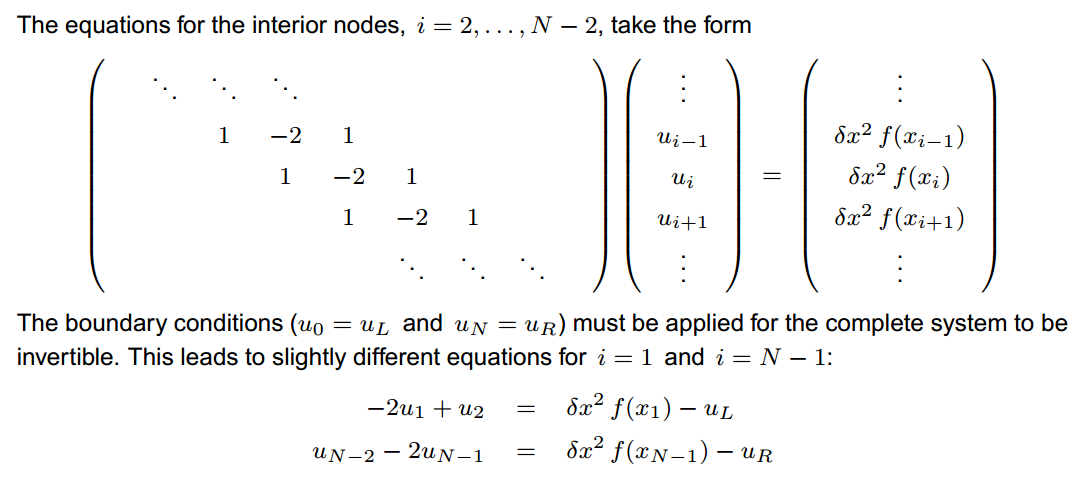
\includegraphics[scale=0.45]{figures/bvp-system.png}
	\caption{Boundary Value Problem System of Equations Structure}
	\label{fig:bvp-system}
\end{figure}
\begin{equation}
	-2u_1 + u_2 = \delta x^2 f(x_1) - u_L
	\label{eq:bvp-system-1}
\end{equation}
\begin{equation}
	u_{N - 2} - 2u_{N - 1} = \delta x^2 f(x_{N - 1}) - u_R
	\label{eq:bvp-system-2}
\end{equation}

The \textbf{error} of approximations generated from this system is $O(\delta x^2)$.

\subsubsection{Solving Multi-dimensional BVPs}

An example of a multi-dimensional boundary value problem is \textbf{heat diffusion}. This is where you know the temperature at the boundaries of a physical body, and want to know the temperature of the rest of the body in-between the boundaries. The temperature $u(t, x, y, z)$ at time $t$ can be found by solving the PDE in Equation \ref{eq:head-diffusion-pde}, where $k$ is the thermal conductivity, $c$ is the specific heat and $p$ is the density of the body. this section will assume those three values are constant.

\begin{equation}
	\frac{\partial u}{\partial t} = \frac{k}{cp} \left( \frac{\partial^2 u}{\partial^2 x} + \frac{\partial^2 u}{\partial^2 y} + \frac{\partial^2 u}{\partial^2 z}  \right)
	\label{eq:head-diffusion-pde}
\end{equation}

If temperature does not change as time progress, then the problem represents a \textbf{steady state} and $\frac{\partial u}{\partial t} = 0$. So if we're only really concerned with space, we can assume the temperature does not change over time and simplify to Equation \ref{eq:laplace}. This equation is known as the \textbf{Laplace Equation}.

\begin{equation}
	\frac{\partial^2 u}{\partial x^2} + \frac{\partial^2 u}{\partial y^2} + \frac{\partial^2 u}{\partial^2 z^2} = 0
	\label{eq:laplace}
\end{equation}

Other sources/sinks of heat can be added to the physical body. If this is the case, then the \textbf{Poisson Equation} shown in Equation \ref{eq:poisson} is used. 

\begin{equation}
	\frac{\partial^2 u}{\partial x^2} + \frac{\partial^2 u}{\partial y^2} + \frac{\partial^2 u}{\partial z^2} = f(x, y, z)
	\label{eq:poisson}
\end{equation}

To approximate these values on a computer, the problem must be discretised. \textbf{Finite Differences} is one way of doing this. It evenly splits up the region between the two boundaries using $N$ uniformly spaced nodes, defining an equation (Equation \ref{eq:finite-differences-1d-node} for each node $i = 1, 2, ..., N - 1$. Doing so results in a system of equations to solve, which finds the values at every point $i$. Figure \ref{fig:finite-differences} illustrates the finite difference approximation of a 1D problem.

\begin{figure}
	\centering
	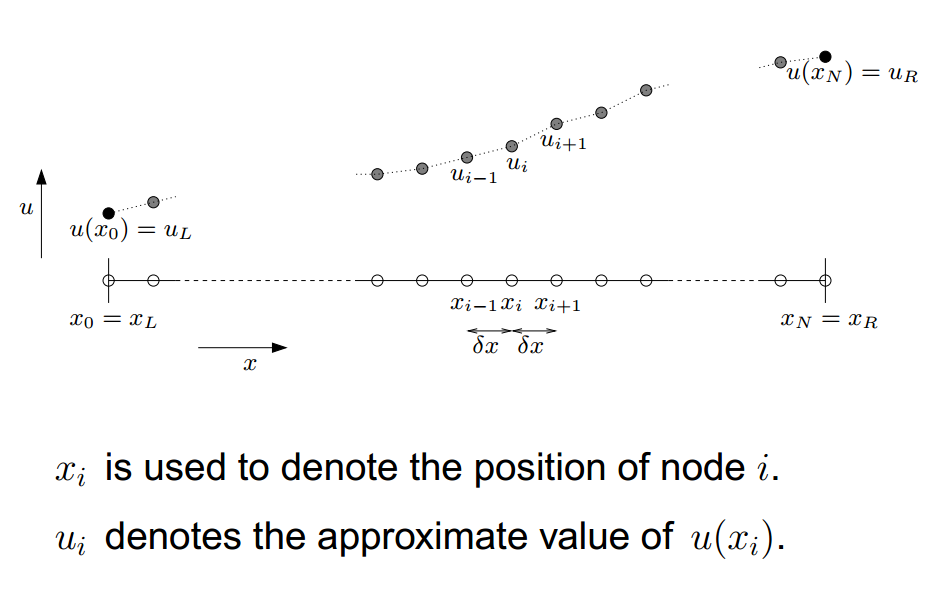
\includegraphics[scale=0.35]{figures/1d-finite-differences.png}
	\caption{Finite Difference Approximation in One Dimension}
	\label{fig:finite-differences}
\end{figure}

\begin{equation}
	{\left( \frac{\partial^2 u}{\partial x^2}\right)}_i \approx \frac{u_{i+1} - 2u_i + u_{i - 1}}{\delta x^2} 
	\implies
	u_{i - 1} - 2u_i + u{i + 1} = \delta x^2 f(x_i)
	\;\;\;\;\;\;\;\; \forall 
	i \in \lbrace 1, 2, ..., N - 1 \rbrace
	\label{eq:finite-differences-1d-node}
\end{equation}

The resultant system is shown in Equation \ref{eq:finite-differences-1d-system}. This is a \textbf{tridiagonal matrix} which can be solved quickly using Gaussian Elimination (since the forward elimination step is not required). The equations at each end need to be different, due to the \textbf{Dirichlet boundary condition}.

Instead of just concerning one dimension, the Poisson equation can be applied to two spatial dimensions (\ref{eq:poisson-2d}). A discretised form can be derived, which results in two equations (Equation \ref{eq:poisson-2d-approx}). Instead of a uniformly split up line, the problem is now uniform 2D mesh like the one in Figure \ref{fig:2d-finite-differences-mesh}.

\begin{equation}
	\frac{\partial^2 u}{\partial x^2} + \frac{\partial^2 u}{\partial y^2} +  = f(x, y)
	\;\;\;\;\;\;\;\;\;\; \forall (x, y) \in \Omega
	\label{eq:poisson-2d}
\end{equation}

\begin{equation}
	{\left( \frac{\partial^2 u}{\partial x^2} \right)}_{i,j} \approx \frac{u_{i + 1,j} - 2u_{i,j} + u_{i - 1,j} }{\delta x^2}
	\;\;\;\;\;\;\;\;\;\; 
	{\left( \frac{\partial^2 u}{\partial y^2} \right)}_{i,j} \approx \frac{u_{i,j+1} - 2u_{i,j} + u_{i,j-1} }{\delta y^2}	
	\label{eq:poisson-2d-approx}
\end{equation}

If the interval between each node is the same for both the X and Y dimensions ($\delta x = \delta y = h$), then an even simpler form that uses a single equation can be used:
\begin{equation}
	f(\vec{x}_{i,j}) = \frac{u_{i + 1,j} - 2u_{i,j} + u_{i - 1,j} }{\delta x^2} + \frac{u_{i,j+1} - 2u_{i,j} + u_{i,j-1} }{\delta y^2}	
	\label{eq:poisson-2d-approx-uniform}
\end{equation}

\begin{figure}
	\centering
	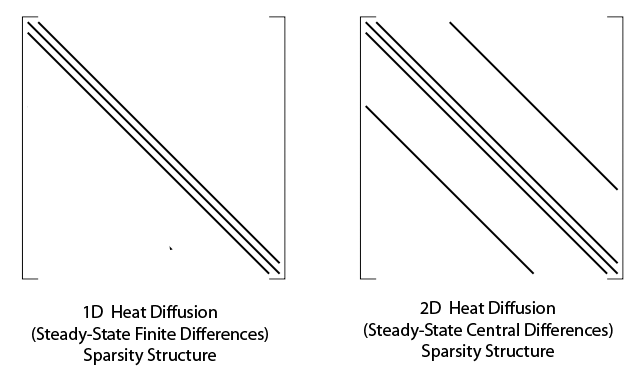
\includegraphics[scale=0.35]{figures/heat-diffusion-sparsity-structures.png}
	\caption{Sparsity Structure of 1D and 2D Systems using Poisson Equation (therefore, the heat diffusion problem also has this problem)}
	\label{fig:poisson-1d-and-2d-sparsity}
\end{figure}

The dimensions of resultant system is $(N - 1)^2 \times (N - 1)^2$ and has the sparsity structure shown in Figure \ref{fig:poisson-1d-and-2d-sparsity}. See Section \ref{sec:heat-diffusion-parallel} for discussion on how to parallelise the problem of solving this system.

\subsubsection{Initial-Boundary Value Problems}

\textbf{Initial-Boundary Value problems (IBVP)} model situations which not only vary in space, but in time. BVPs typically just model variance in space, meaning they model steady-state situations (like the heat difussion problem). IBVPs on the other hand provide a way of describing dynamic models that form some variation in time. IBVPs allow you to simulate pretty much anything, such as:
\begin{itemize}
	\item weather across the globe
	\item water flow/current produced by a swimmer to find optimal strokes
	\item nuclear bomb simulations
\end{itemize}

Partial differential equations are used to describe IBVPs. In order to predict the evolution of the system, it requires the \textbf{initial} boundary values (as the boundary values can now change over time).

In its own general form, IBVPs which vary in \textbf{one spatial dimension} $x$ can be represented with the PDE shown in Equation \ref{eq:ivbp-general-1d}. Equation \ref{eq:ivbp-general-1d} shows a more generalised PDE for \textbf{multiple spatial dimensions}.

\begin{equation}
	\frac{\partial u}{\partial t} + \lambda\frac{\partial u}{\partial x} = \epsilon \frac{\partial^2 u}{\partial x^2} + r(u)
	\label{eq:ivbp-general-1d}
\end{equation}

\begin{equation}
	\frac{\partial u}{\partial t} + \vec{\lambda} \cdot \vec{\bigtriangledown}u = \epsilon \cdot \vec{\bigtriangledown^2}u + r(u)
	\label{eq:ivbp-general-multid}
\end{equation}

\begin{itemize}
	\item $\lambda\frac{\partial u}{\partial x}$  represents \textbf{advection}. Advection represents movement through the spatial domain. $\lambda$ describes the \textbf{direction and velocity} (through sign and magnitude respectively) of the information is flowing. Since velocity can change over time, $\lambda$ can vary over time. $\frac{\partial u}{\partial t} + \lambda\frac{\partial u}{\partial x} = 0$ is used when a problem just has advection/movement.
	\item $\epsilon \frac{\partial^2 u}{\partial x^2}$ represents \textbf{diffusion}. This \textbf{smooths} out the value of $u$. The speed at which the information is smoothed out depends on the magnitude of $\epsilon$, which should not be negative. If just diffusion is used, then $\frac{\partial u}{\partial t} + \epsilon\frac{\partial^2 u}{\partial x^2}$ is used when a problem just has advection/movement. Heat diffusion is an example of this.
	\item $r(u)$ represents \textbf{reaction}. This represents the creation, destruction and conversion of different components of the system, and can be any arbitrary function. Just reaction would be $\frac{\partial u}{\partial t} = r(u)$.
\end{itemize}
Figure \ref{fig:advection-diffusion-behaviour} shows the behaviour of the model as $\lambda$ and $\epsilon$ are changed. Changing $\lambda$ changes the position of the situation in the spatial domain and changing $\epsilon$ determines how much the behaviour is smoothed out.

TODO: diagrams showing behaviour of the different stuff (slide 10)

\paragraph{\textbf{NOTE:}} Leaving the time-derivative out from any of theese equations leave \textbf{steady-state equations} that are related to BVPs. For example, if you left the time derivative out of the diffusion equation, then it would represent the heat diffusion BVP.
\paragraph{}

\textbf{Method of lines} is a common approach to approximating time-dependant PDEs, such as IBVPs. It requires the following steps:
\begin{enumerate}
	\item discretise spatial dimension(s) using \textbf{finite differences}
	\item discretise time using \textbf{explicit time-stepping with the forward Euler scheme}
	\item convert disrectisation into matrix/vector form so it can be solved a system of equations
\end{enumerate}

Central differences can be used to approximate the spatial derivative(s). Equation \ref{eq:ibvp-spatial-approx} shows such an approximation for \textbf{both} advection and diffusion. This means each internal node of the problem's mesh gets the \textbf{time-dependant} formula shown in Equation \ref{eq:ibvp-spatial-approx-node}.

\begin{multline} \\
	{\left( \frac{\partial u}{\partial x} \right)}_i \approx \frac{u_{i + 1} - u_{i - 1}}{2\delta x} \\
	{\left( \frac{\partial^2 u}{\partial x^2} \right)}_i \approx \frac{u_{i + 1} - 2u_i + u_{i - 1}}{\delta x^2} \\
	\label{eq:ibvp-spatial-approx}
\end{multline}

\begin{multline} \\
	\dot{u}_i = \lambda \frac{u_{i + 1} - u_{i - 1}}{2\delta x} + \epsilon \frac{u_{i + 1} - 2u_i + u_{i - 1}}{\delta x^2} + r(u-i) \\
	\dot{u}_i = g_i(t, u(t)) \\
	\label{eq:ibvp-spatial-approx-node}
\end{multline}

Note that $\dot{u}$ means a spatial approximation which depends on continuous time (i.e. time has not been discretised yet). Using the forward Euler scheme to discretise $\dot{u}$ gives:
\begin{multline}\\
	g(t, u(t)) \approx \frac{u(t + \delta t) - u(t)}{\delta t} \implies \\
	u^{n+1} = u^n + \delta t g(t^n, u^n) \\
\end{multline}

This makes the final advection-diffusion-reaction with central differences in space at point $i$ and time $n$ the formula in Equation \ref{eq:ibvp-final-discrete-form}. The \textbf{initial conditions $u^0$}, or values for each spatial point $i$ at time $0$, must be specified. Boundary conditions are also required at $x_L$ and $x_R$.

\begin{equation}
	u_i^{n+1} = u_i^n - \frac{\lambda \delta t}{2 \delta x}(u_{i+1}^n - u_{i-1}^n) + \frac{\epsilon \delta t}{\delta x^2}(u_{i+1}^n - 2u_i^n + u_{i-1}^n) + \delta tr(u_i^n)
	\label{eq:ibvp-final-discrete-form}
\end{equation}

Since \textbf{explicit time-stepping} is being used, the scheme is only \textbf{conditionally stable}. There is limit to how far ahead in time the next approximation can be made! The error in the scheme is $O(\delta t + \delta x^2)$. To achieve unconditional stability and predict ahead as far as we want in time, \textbf{upwinding} and \textbf{backward Euler scheme} (implicit time-stepping) is required for the spatial and time discretisation respectively (not central differences or the forward Euler scheme). Note that upwinding \textbf{increases error} but ensures stability. Equations \ref{eq:ibvpupwinding-discretisation} and \ref{eq:ibvp-backward-euler} show these spatial and time discretisations, result in the final approximation equation shown in \ref{eq:ivbp-approx-final2}.

\begin{multline}\\
	{\left( \frac{\partial u}{\partial x} \right)}_i \approx \frac{u_i - u_{i - 1}}{\delta x} \;\;\;\;\; when \;\; \lambda \geq 0 \\
	{\left( \frac{\partial u}{\partial x} \right)}_i \approx \frac{u_{i+1} - u_{i}}{\delta x} \;\;\;\;\; when \;\; \lambda < 0 \\
	\label{eq:ibvpupwinding-discretisation} 
\\ \end{multline}

\begin{multline}\\
	\frac{u(t + \delta t) - u(t)}{\delta t} \approx g(t + \delta t, u(t + \delta t)) \\
	\implies u^{n+1}= u^n + \delta t g(t^{n+1}, u^{n+1})
	\label{eq:ibvp-backward-euler}
\\ \end{multline}

\begin{equation}
	\frac{u_i^{n + 1} - u_i^n}{\delta t} = -\lambda \frac{u_{i+1}^{n+1} - u_{i-1}^{n+1}}{2 \delta x} + \epsilon \frac{u_{i+1}^{n+1} - 2u_{i}^{n+1} + u_{i-1}^{n+1}}{\delta x^2} + r(U_i^{n+1})
	\label{eq:ivbp-approx-final2}
\end{equation}

As before, the initial conditions $u^0$ must be specified and Dirichlet boundary conditions can be imposed by fixing boundary values $u(X_L) = u_L$ and $u(X_R) = u_R$. 

As always, these equations form a system $Ax = b$ which can be solved. Assuming $r(u) = 0$, the sparsity pattern of the matrix $A$ IBVPs \textbf{matches} the pattern of the \textbf{BVP of the steady-state} problem, which is shown in Figure \ref{fig:bvp-ibvp-sparsity} (however, the coefficients are complex in IBVPs). Each timestep requires solving the system of equations.

TODO: sparsity structure diagram of BVPs and IBVPs.

\subsection{Sparse Systems}

The computational cost of Gaussian Elimination for a dense matrix is $O(n^3)$ and the storage cost is $O(n^2)$. This is tractable for small $n$, but rapidly becomes too expensive. It is common that there are many zero coefficients in the system of equations, which means there are many zeros in matrix $A$ of $Ax = b$. This means $A$ is a \textbf{sparse matrix} and the $O(n^2)$ storage is unnecessary as the majority of the entries are 0.

\subsubsection{Storing Sparse Matrices}

\textbf{Sparse data storage} removes entries that the matrix that are known to be zero. the nonzero entries must be stored efficiently. Two storage approaches to sparse matrix storage ill be discussed here. Let $n$ be the number of rows and columns in matrix and $n_{nz}$ be the number of non-zero entries.

\textbf{Coordinate format (AIJ)} uses three arrays, each of length $n_{nz}$ to store:
\begin{enumerate}
	\item the row indices of the non-zeros
	\item the column indices of the non-zeros
	\item the \textit{values} of the non-zeros
\end{enumerate}
Therefore, the memory requirement is $3n_{nz}$. Table \ref{tab:coordinate-format} shows an example of the coordinate format representation. row[1] = 1, column[1] = 2 and value[1] = $2$ would mean that the value of the element at row one, column two of the matrix is 2.

\begin{table}
	\centering
	\begin{tabular}{|l|llllllllllllll|}
		\hline
		\textbf{Row} & 1 & 1 & 1 & 1 & 2 & 2 & 2 & 2 & 2 & 3 & 3 & 3 & 3 & ... \\
		\hline
		\textbf{Column} & 1 & 2 & 9 & 10 & 1 & 2 & 3 & 10 & 11 & 2 & 3 & 4 & 11 & ... \\
		\hline
		\textbf{Value} & $M_{1,1}$ & $M_{1,2}$ & $M_{1,9}$ & $M_{1,10}$ & $M_{2,1}$ & $M_{2,2}$ & $M_{2,3}$ & $M_{2,10}$ & $M_{2,11}$ & $M_{3,2}$ & $M_{3,3}$ & $M_{3,4}$ & $M_{3,11}$ & ... \\
		\hline
	\end{tabular}
	\caption{Coordinate Format representation for matrix $M$, which uses three arrays of size $n_{nz}$ (NOTE: indices are starting from 1 here)}
	\label{tab:coordinate-format}
\end{table}

\textbf{Compressed Sparse Row Format (CSR)} maintains an array of size $N$, which contains an offset for each of the $N$ rows of the matrix. These offsets are \textbf{indices into the column array} which corresponding to the first entry of that row. Another array of size $n_{nz}$ contains the \textbf{column indices} of the non-zero entries and there is a final array of size $n_{nz}$ which contains the values of the non-zeros.. The latter two arrays are the same as the latter two arrays of the coordinate format.

The memory requirement for such a scheme is $2n_{nz} + n + 1$, because all $n$ rows have an offset entry in the rows array. rows[2] = 10, column[10] = 20, value[10] = 5 would mean that the matrix entry at row 2, column 10 has a value of 5.

\begin{table}
	\centering
	\begin{tabular}{|l|llllllllllllll|}
		\hline
		\textbf{Row} & 1 & 5 & 10 & 14 & 19 & 23 & ... &&&&&&& \\
		\hline
		\textbf{Column} & 1 & 2 & 9 & 10 & 1 & 2 & 3 & 10 & 11 & 2 & 3 & 4 & 11 & ... \\
		\hline
		\textbf{Value} & $M_{1,1}$ & $M_{1,2}$ & $M_{1,9}$ & $M_{1,10}$ & $M_{2,1}$ & $M_{2,2}$ & $M_{2,3}$ & $M_{2,10}$ & $M_{2,11}$ & $M_{3,2}$ & $M_{3,3}$ & $M_{3,4}$ & $M_{3,11}$ & ... \\
		\hline
	\end{tabular}
	\caption{Compressed Sparse Row format representation for matrix $M$}
	\label{tab:compressed-sparse-row-format}
\end{table}

\subsubsection{Structured Sparsity and Banded Matrices}

For structured meshes, like the mesh for the heat diffusion problem, there is clearly a structure to the sparsity pattern in the matrix $A$. For example, one-dimensional heat diffusion has a tri-diagonal matrix (three diagonals of non-zero values). Two-dimensional heat diffusion has five diagonals of non-zeros.  This is equivalent to the sparsity structure of 1D and 2D Poisson equations, as shown on Figur e \ref{fig:poisson-1d-and-2d-sparsity}.

Rather than store the whole matrix, or even use one of the sparse matrix representations discussed previously, we can store each diagonal as a vector. This means we only need to use 3 $n$-sized vectors for 1D heat diffusion and 5 $n$-sized vectors for two-dimensions!

In fact, when the matrix structure is derived from a structured lattice, the off-diagonal non-zero entries can always be easily stored as arrays. Figure \ref{fig:banded-matrix} shows a \textbf{banded matrix}. Banded matrices store the non-zero "bands" of a sparse matrix as arrays, resulting in a two-dimensional array.

\begin{figure}
	\centering
	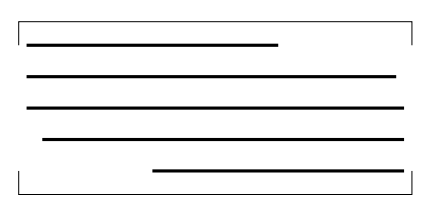
\includegraphics[scale=0.4]{figures/banded-matrix.png}
	\caption{Banded matrix containing five vectors for the five non-zero diagonals of 2D heat diffusion}
	\label{fig:banded-matrix}
\end{figure}

\subsubsection{Thomas Algorithm}

The \textbf{Thomas algorithm} is an efficient implementation of Gaussian elimination for a \textbf{tri-diagnonal matrix}. Both the forward elimination and back substitution steps can be done in $O(n)$ operations each, meaning a system with a tri-diagonal sparsity structure can be solved with a direct method in $O(n)$ time).

TODO

\subsubsection{Unstructured Meshes}

The matrix for the system of equations has non-zeros wherever the nodes are connected, including on the diagonal. Figure \ref{fig:unstructured-mesh-sparsity} shows the sparsity structure of a particular unstructured mesh. You can see how there are non-zeros on the diagonal and whenever there's node connectivity ($A_{1,2}$ and $A_{2,1}$ have non-zero entries because nodes 1 and 2 are connected). Since the node connectivity is always symmetric, the \textbf{sparsity structure is always symmetric}. However, while the actual coefficients may both be non-zero, they might not be same, so $A$ is not necessarily a symmetric matrix.
\begin{figure}
	\centering
	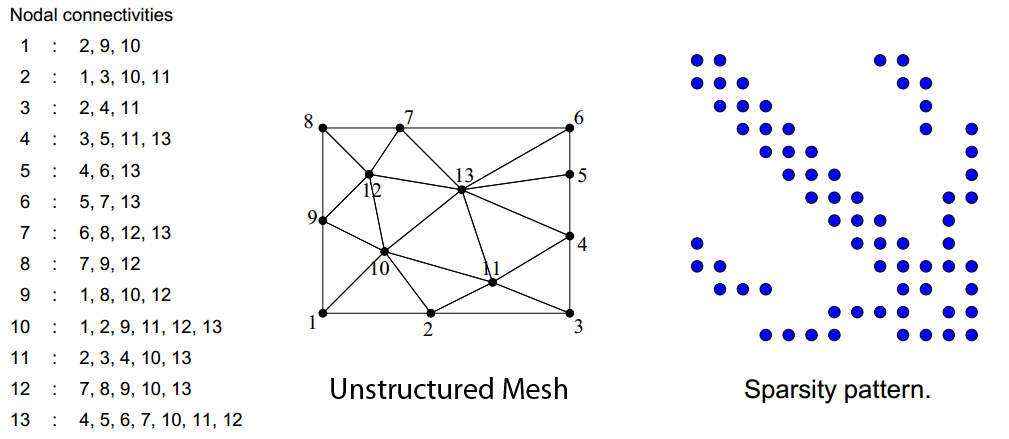
\includegraphics[scale=0.4]{figures/unstructurered-sparsity-structure.png}
	\caption{Unstructured mesh shown with node connectivities and the corresponding sparsity structure of the mesh's system}
	\label{fig:unstructured-mesh-sparsity}
\end{figure}

\subsubsection{Bandwidth}

\textbf{Sparse matrix-vector multiplications} can have poor computational performance because random access of the vector $x$ can cause \textbf{cache misses}. This is because the elements in $x$ may not be accessed sequentially, but it more scattered, unpredictable order, due to the sparsity of the matrix.

The \textbf{bandwidth} of a matrix $A$ is the minimum value of $m$ for which $a_{i,j} = 0$ $\forall |i - j| > m$£. That is, bandwidth is the \textbf{distance from the diagonal to the furthest non-zero element} (the sum of horizontal and vertical distance).

\textbf{Re-ordering} the rows and columns of the matrix so that the non-zero entries close to the diagonal increases efficiency because it exploits \textbf{cache locality} to get more cache hits. This also helps reduce \textbf{fill-in}, which is when new non-zero elements are introduced into the matrix between nodes which are not connected (typically caused by turning a matrix into upper/lower triangular form in order to solve).

\subsubsection{Cuthill-McKee Ordering}

TODO: describe algorithm

TODO: give steps

TODO; give example

TODO: mention fill-in

\section{Meshes}

A \textbf{mesh} is essentially a graph. It consists of nodes (vertices) which are connected by edges. Each node represents some value (e.g. value at a point in space or time) in a problem and an edge between two nodes represents a dependency between the two values (e.g. neighbouring points in heat diffusion plate).

\subsection{Mesh Representation}
\label{sec:mesh-representation}

Meshes are made of simple components. For one, two and three dimensional meshes these components are:
\begin{itemize}
	\item \textbf{1D} -- nodes and elements
	\item \textbf{2D} -- nodes, edges and elements
	\item \textbf{3D} -- nodes, edges, faces and elements
\end{itemize}
Figure \ref{fig:mesh-components} illustrates and labels these components for 2D and 3D meshes.

\begin{figure}
	\centering
	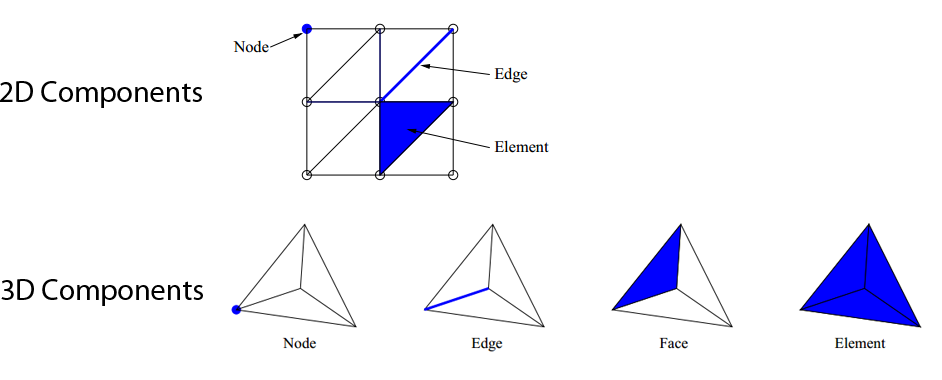
\includegraphics[scale=0.4]{figures/unstructured-mesh-components.png}
	\caption{Components of 2D and 3D unstructured meshes}
	\label{fig:mesh-components}
\end{figure}

In its smallest form, a mesh/graph can be represented using just two lists:
\begin{enumerate}
	\item list of nodes (and their positions in space if required)
	\item list of triangles, specified by node indices
\end{enumerate}

Table \ref{tab:mesh-representation} shows the node and triangle list for the 2D mesh in Figure \ref{fig:mesh-representation}.

\paragraph{}

Note that in two dimensions:
\begin{itemize}
	\item each \textbf{edge} has \textbf{two nodes}
	\item each \textbf{triangle} has \textbf{three nodes}
	\item each \textbf{triangle} has \textbf{three edges}
	\item each \textbf{internal edge} is in \textbf{two triangles}
\end{itemize}
However:
\begin{itemize}
	\item each \textbf{node} can be in \textbf{different numbers of triangles}
\end{itemize}
How many triangles a node belongs to can greatly affect the mesh's behaviour and overall performance (see Section \ref{sec:mesh-quality}).

\begin{figure}
	\centering
	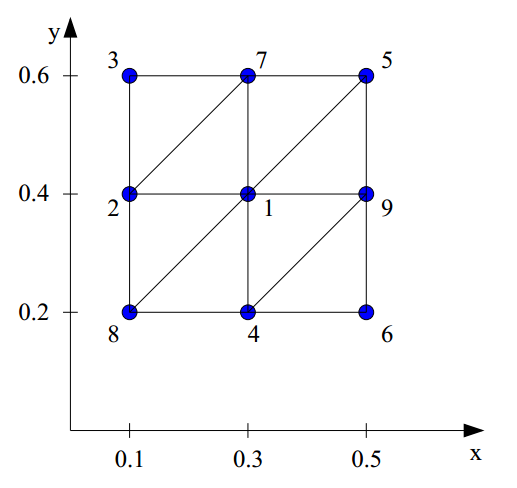
\includegraphics[scale=0.4]{figures/unstructured-mesh-example.png}
	\caption{Unstructred mesh generated from Table \ref{tab:mesh-representation}}
	\label{fig:mesh-representation}
\end{figure}

\begin{table}
	\centering
	\begin{tabular}{|l|l|l|l|l|l|}
		\hline
		\multicolumn{3}{|c|}{\textbf{List of Nodes}} & \multicolumn{3}{|c|}{\textbf{Triangles}} \\
		\hline
		\multicolumn{3}{|l|}{9} & \multicolumn{3}{|l|}{8} \\		
		\hline
		1) & 0.3 & 0.4 & 8 & 4 & 1 \\
		2) & 0.1 & 0.4 & 4 & 6 & 9 \\
		3) & 0.1 & 0.6 & 4 & 9 & 1 \\
		4) & 0.3 & 0.2 & 8 & 1 & 2 \\
		5) & 0.5 & 0.6 & 2 & 7 & 3 \\
		6) & 0.5 & 0.2 & 2 & 1 & 7 \\
		7) & 0.3 & 0.6 & 1 & 9 & 5 \\
		8) & 0.1 & 0.2 & 1 & 5 & 7 \\
		9) & 0.5 & 0.4 & & & \\
		\hline
	\end{tabular}
	\caption{Representation of arbitrary 2D mesh shown in Figure \ref{fig:mesh-representation}}
	\label{tab:mesh-representation}
\end{table}

\paragraph{\textbf{NOTE:}} Always number a triangle's nodes in an \textbf{anti-clockwise} fashion. An orientation is always assumed when using existing solvers/algorithms, so it is best to be consistent . This is similar to using an anti-clockwise winding order for the faces of 3D meshes in real-time graphics.

\subsection{Structured/Unstructured Problems}
\label{sec:structured-unstructured-problems}

The majority of problems considered in this document have used regular, structured meshes (e.g. heat diffusion). These structured meshes have had uniform mesh spacing, which means we can use \textbf{finite difference approximations}. A \textbf{structured} mesh is one which has a determinable structure, such as every node having exactly 4 neighbours (except for boundary nodes). A \textbf{regular} mesh is a structured mesh where the spacing between each node is uniform (the same). Figure \ref{fig:regular-structured-meshes} shows examples of these.

\begin{figure}
	\centering
	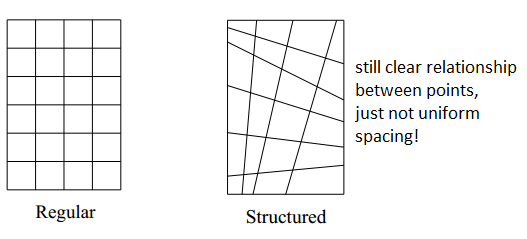
\includegraphics[scale=0.6]{figures/regular-structured-mesh.png}
	\caption{A regular and structured mesh}
	\label{fig:regular-structured-meshes}
\end{figure}

If a problem produces a structured mesh, then it is considered a \textbf{structured problem}. An \textbf{unstructured problem} is one in which the mesh covers a domain \textit{without} regular arrangements of points or connections. Specifically, the mesh forms a \textbf{connected graph} where the nodes are connected by \textbf{non-crossing edges}. \textbf{Hanging nodes}, where a node of a triangle is in the \textit{middle} of another triangle's edge, are usually avoided in unstructured problems too. See Figure \ref{fig:unstructured-meshes} for examples of typical unstructured meshes and hanging nodes).

\begin{figure}
	\centering
	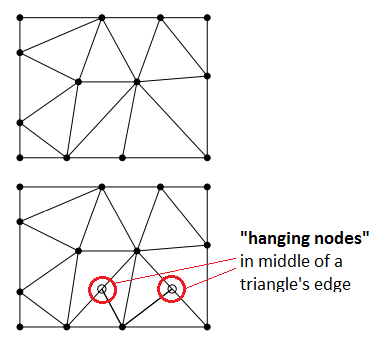
\includegraphics[scale=0.5]{figures/unstructured-mesh-examples.png}
	\caption{Unstructured Meshes}
	\label{fig:unstructured-meshes}
\end{figure}

In two dimensions, \textbf{triangular meshes} are typically used. Tessellation using triangles is well understood, as any straight-edged shape can be decomposed into triangles. There are usually multiple ways to decompose a mesh into triangles (i.e. no unique decomposition). Each way results in a different solution as it gives a specific orientation to the data. Quadrilaterals are use occassionally if it makes computation more efficient/accurate for the problem at hand. In 3D, tetrahedra or hexahedra are often used.

Consider the two-dimensional Poisson equation given in Equation \ref{eq:poisson-2d}. Its central difference discretisation gives:
\begin{equation}
u_{i+1,j} + u_{i,j+1} + u_{i-1,j} + u_{i,j-1} - 4u_{i,j} = h^2f(\vec{x_i,j})
\end{equation}
which leads to the Jacobi iteration of the form:
\begin{equation}
u_{i,j}^{(k+1)} = \frac{1}{4} \left( u_{i-1,j}^{(k)} + u_{i,j-1}^{(k)} + u_{i+1,j}^{(k)} + u_{i,j+1}^{(k)} - h^2f(\vec{x_i,j}) \right)
\end{equation}
On a structured mesh, it is simple to compute this because the \textbf{indices} automatically pick the correct neighbours of a node to average. It takes advantage of the \textit{known} structure of the mesh.

With unstructured data there is no longer a regular grid of $(N - 1) \times (N - 1)$ nodes. Mutlidimensional arrays can no longer be used, the adjacent nodes are not automatically known and the nodes are a fixed distance apart. This is when the mesh must be represented in a more complex way, such as the representation given in in Section \ref{sec:mesh-representation} is required.

\subsection{Process of Solving Unstructured Problems}

The steps of the overall process of solving an unstructured problem, after deriving a numerical model, are listed below. Later sections will go into detail about these specific steps.
\begin{enumerate}
	\item Construct the mesh (Section \ref{sec:mesh-generation})
	\item Partition the nodes between processes  (Section \ref{sec:mesh-partitioning})
	\item Load the mesh geometry and connectivity from files and store in memory (Section \ref{sec:mesh-loading})
	\begin{enumerate}
		\item Node indexing is automatic from loaded order
		\item Pre-allocate memory for subsequent computations
		\item Pre-compute fixed information about the mesh (e.g. number of nodes, edges, triangles, degree of each node, etc.
	\end{enumerate}
	\item Build the sparse matrix structure and contents
	\item Solving the resulting matrix system
	\item Estimate errors and adapt the mesh accordingly (Section \ref{sec:adaptive-meshes})
	\item Repartition the nodes and go back to step 5
\end{enumerate}

\subsection{Mesh Generation}
\label{sec:mesh-generation}

Less data is required to construct regular and structured meshes. For a uniform grid for example, all you need are the positions of the two opposite corners and the number of divisions in the $x$ and $y$ directions (number of columns and rows). For unstructured meshes with $N$ points, $B$ of which are on the boundary there are:
\begin{itemize}
	\item $2N - 2 - B$ triangles
	\item $3N - 3 - B$ edges
\end{itemize}
in \textbf{any triangulation}. This requires much more information to construct than a uniform grid, meaning more memory is required. However, this property makes pre-allocating enough memory to fit the unstructured mesh easy, providing you know $N$ and $B$.

\subsubsection{Mesh Quality}
\label{sec:mesh-quality}

Unstructured meshes can be \textbf{constructed from a point cloud} like the one on the left of Figure \ref{fig:unstructured-mesh-construction}. Every point cloud can be triangulated in many different ways, producing different meshes. There needs to a be a way of \textbf{assessing} which mesh is the best. Intuitively, mesh A in Figure \ref{fig:unstructured-mesh-construction} looks better than mesh B, because the triangles roughly match in size and are closer to equilateral triangles. Additionally, the points closest to each other are connected. This prevents the \textbf{orientation} biasing the output as much.

\begin{figure}
	\centering
	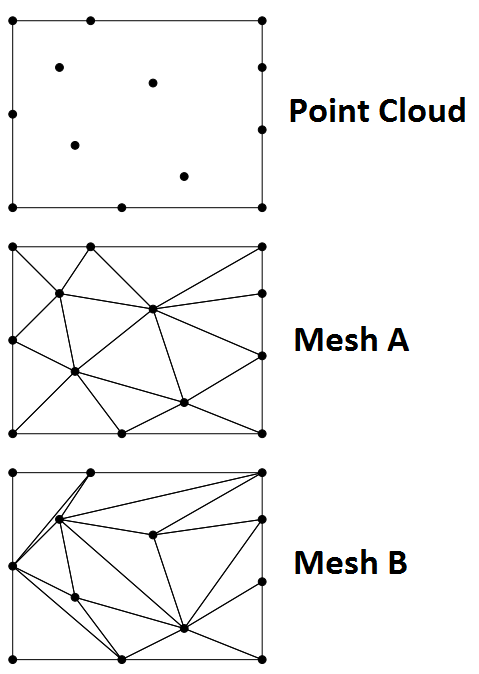
\includegraphics[scale=0.35]{figures/mesh-quality-example.png}
	\caption{Two ways of constructing mesh from point cloud}
	\label{fig:unstructered-mesh-construction}
\end{figure}

Equations \ref{eq:mesh-quality-1} and \ref{eq:mesh-quality-2} are two quality measures often used when assessing meshes. Higher values mean better quality meshes. Equilateral triangles are generally best, so these measures allow you to try and \textbf{maximise} the smallest angle in the mesh and/or \textbf{minimise} the largest.

The second measure outputs area divided by the sum of the length of each side, which prevents tall thin triangles. The first measure returns the smallest angle, which can be used to prevent triangles where the length of the sides vary in length.

\begin{equation}
	Q_1 = \min \lbrace \theta_1, \theta_2, \theta_3 \rbrace
	\label{eq:mesh-quality-1}
\end{equation}

\begin{equation}
	Q_2 = \frac{A}{l_1^2 + l_2^2 + l_3^2}
	\label{eq:mesh-quality-2}
\end{equation}

\subsubsection{Edge Swapping}

Edges connected two nodes can be swapped to improve mesh quality. Look at the triangulation in Figure \ref{fig:edge-swapping}. The edge between $r_1$ and $r_3$ is deemed \textbf{illegal} if $\min \lbrace a, b, c, d, e, f \rbrace < \min \lbrace A, B, C, D, E,F \rbrace$.  Illegal edges should be swapped for other edges such that the mesh is still triangulated. This is because the alternative triangulation resulted in a higher quality mesh (by quality measure $Q_1$).

Steps:
\begin{enumerate}
	\item Pick two triangles
	\item Compute angles of both triangles $a, b, c$ and $d, e, f$
	\item Swap the connecting edge of the two triangles
	\item Compute angles of resulting triangles $A, B, C$ and $D, E, F$
	\item If $\min \lbrace a, b, c, d, e, f \rbrace < \min \lbrace A, B, C, D, E,F \rbrace$, the original triangulation is \textbf{illegal}, so make the swap \textbf{permanent}.
	\item Repeat until there are no illegal edges (swapping edges may produce new illegal edges). At this point, a \textbf{Delaunay triangulation} has been achieved.
\end{enumerate}

\subsubsection{Voronoi Tesselation}

\textbf{Voronoi tessellation} divides the mesh area into regions using lines that are \textbf{equidistant from pairs of points}. Doing this produces a Voronoi diagram, like the one shown in Figure \ref{fig:voronoi-tesselation} for the mesh $S = \lbrace r_1, r_2 \rbrace$.

\begin{figure}
	\centering
	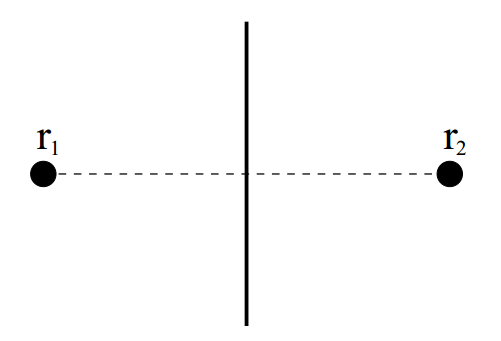
\includegraphics[scale=0.35]{figures/voronoi-basic-diagram.png}
	\caption{Voronoi diagram of $S = \lbrace 1, 2 \rbrace$}
	\label{fig:unstructered-mesh-construction}
\end{figure}

A \textbf{Voronoi cell} $V(r_i)$ is the region containing mesh vertex $r_i$. A \textbf{Voronoi vertex} $v_p$ is equidistant from the three nearest nodes $r_i$, $r_j$ and $r_k$. The circle centred at $v_p$, which touches $r_i$, $r_j$ and $r_k$ on the edge of the circle, must contain \textbf{no other nodes}. These vertices are at the points where three region edges intersect, or at the boundary of the regions. Figure \ref{fig:voronoi-vertex} shows the construction of a single Voronoi vertex from a mesh with three points, with each component of the diagram labelled. Figure \ref{fig:voronoi-diagram} shows an entire Voronoi diagram, illustrating how the circles centred at Vorionoi vertices only contain the three mesh vertices used to construct said Voronoi vertex.

\begin{figure}
	\centering
	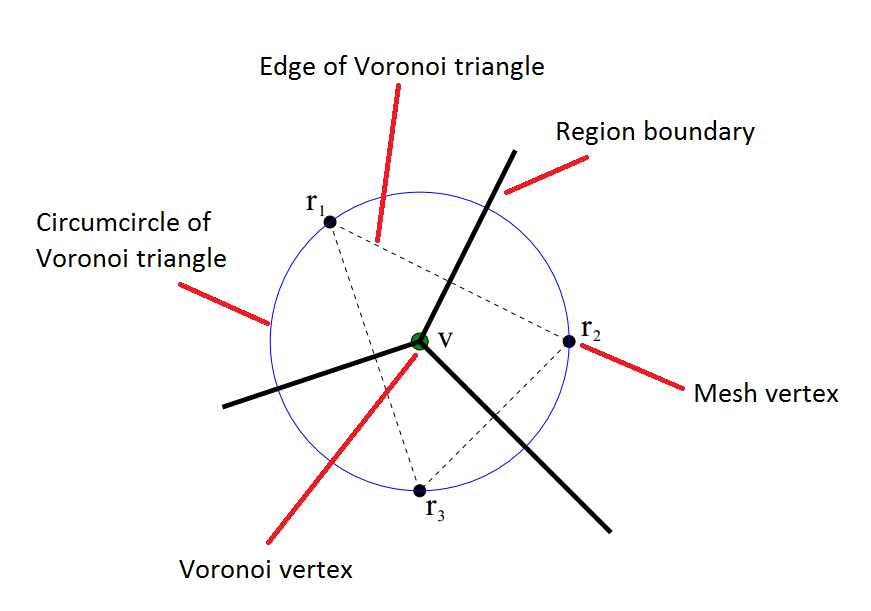
\includegraphics[scale=0.45]{figures/voronoi-vertex.png}
	\caption{Voronoi diagram of $S = \lbrace r_1, r_2, r_3 \rbrace$, with each component of the diagram labelled}
	\label{fig:voronoi-vertex}
\end{figure}

\begin{figure}
	\centering
	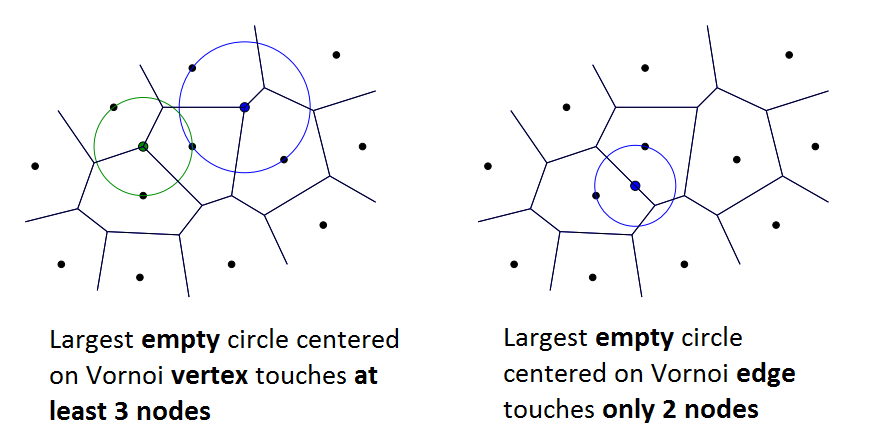
\includegraphics[scale=0.45]{figures/voronoi-diagram.png}
	\caption{Complete Voronoi diagram}
	\label{fig:voronoi-diagram}
\end{figure}

\paragraph{\textbf{NOTE:}} Finding a Voronoi tessellation can be done in $O(n \log n)$ time.

\subsubsection{Dual Graphs and Delaunay Triangulation}

A \textbf{dual graph} of a graph $G$ is a graph whose vertices are the faces of $G$ and there is an edge between two vertices if the two faces in $G$ corresponding to those vertices are adjacent. One can be formed from a Voronoi diagram using the following algorithm.
Let $G = (V, E)$ where $V = \lbrace \rbrace$ and $E = \lbrace \rbrace$.
\begin{enumerate}
	\item for each Voronoi vertex $v_i$, create a vertex $d_i$ at the corresponding position and place it in $V$
	\item if Voronoi vertices $v_i$ and $v_j$ (where $i \neq j$) are contained in \textbf{adjacent Voronoi cells}, then create an edge between $d_i$ and $d_j$.
\end{enumerate}

\textbf{Delaunay triangulation} is a triangulation of a set $P$ of points such that no point in $P$ is inside the cirumcircle (circle growing out of centre) of any triangle. Straightening the edges of the dual graph out and you get a \textbf{Delaunay graph}. If four nodes are on the  circle in the Voronoi diagram, add an extra edge to ensure the graph is a valid Delaunay triangulation.

Figure \ref{fig:vornoi-dual-delaunay} shows how to go from a point cloud to a vornoi diagram and how that can be transformed into a Delaunay triangulation.

\begin{figure}
	\centering
	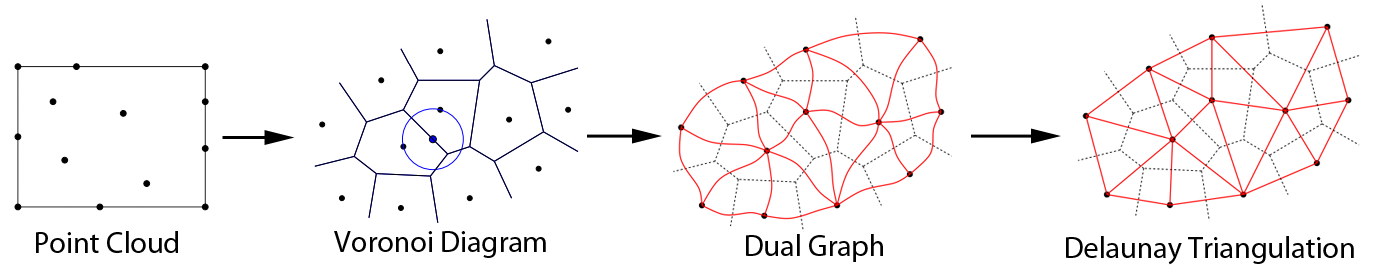
\includegraphics[scale=0.35]{figures/mesh-triangulation-process.png}
	\caption{Process of going from a point cloud to a Delaunay triangulation using Voronoi diagrams and dual graphs}
	\label{fig:vornoi-dual-delaunay}
\end{figure}

Another \textbf{algorithm} to find a Delaunay triangulation from a point cloud $P$ is given below
\begin{enumerate}
	\item Let $P' = \lbrace \rbrace$ and $T' = \lbrace \rbrace$
	\item Choose a \textbf{bounding triangle} $t_b$ from points in $P$ that contains all the points in the cloud and add $t_b$ to $T'$
	\item Choose a point $p$ from $P \setminus P'$
	\item Find the triangle $t \in T'$ containing $p$
	\item Subdivide $t$ into \textbf{three new triangles}, each with $p$ as a vertex
	\item Recursively perform \textbf{edge swapping} until the triangulation is \textbf{legal}
	\item Add $p$ to $P'$
	\item Repeat from step 3 until $P \setminus P' = \emptyset$
	\item Remove \textbf{bounding triangle} $t_b$ from $T'$
\end{enumerate}
Now $T'$ is a Delaunay triangulation for the set of points $P$.

Figure \ref{fig:delaunay-triangulation-example} shows the process of going from a point cloud to a legal Delaunay triangulation, referencing the steps described above.

TODO: big figure listing all steps, with captions from slides to the right of the step and reference to numbered step in algorithm description

\subsubsection{Point Insertion}

Based on the mesh quality measurements discussed, it is still possible to improve a Delaunay triangulation produced by the algorithm in the previous section. \textbf{Point Insertion} is an \textbf{iterative} approach to improving such a triangulation and is given below:
\begin{enumerate}
	\item Find a poor (or even poorest) quality triangle $t$ with points $r_1$, $r_2$ and $r_3$ (using mesh quality measures $Q_1$ and $Q_2$)
	\item Insert the \textbf{cirumcentre} of triangle $t$ as a new mesh node $m$
	\item Add 3 new triangles $r_1t_2m$, $r_2r_3m$, $r_1r_3m$
	\item Recursively perform \textbf{edge swapping} until the triangulation is \textbf{legal}
	\item Repeat from step 1 until the mesh is "good enough"
\end{enumerate}

TODO: figure showing each step, with the caption of each step to the right of it and reference to the steps above

Each step of this algorithm is $O(n)$, apart from finding the triangle that the added point falls within. The information required to perfect the steps can be found in $O(n\log n)$, which is the same complexity as forming the Voronoi tessellation.

\subsubsection{Advancing Front Method}

The quality of the triangulated meshes produced by Delaunay triangulation depends on the set of points given. That is, a poor choice of points could prevent the algorithm from ever finding a good triangulation. An alternative approach which tries to combat this is to define the shape of the \textbf{boundary} with points and then let the algorithm find how points are needed inside the mesh as it builds the triangulation. Letting the user specify the size of the triangles/granularity of the inner nodes to tweak the detail of the mesh is also possible with such approaches.

One such algorithm is the \textbf{Advancing Front Method}, which is a reasonably fast method for producing good triangulations. The steps are as follows:
\begin{enumerate}
	\item Define an external boundary and discretise it to get a set of nodes $P$ and edges which represent the boundary. Let this boundary be the \textbf{initial front} and call it $F$
	\item Let $G = (V, E)$ be a mesh with no nodes or edges
	\item Choose an edge $e = uv$ on $F$ (perhaps the \textbf{shortest})
	\item Choose a position inside the boundary of the mesh and create a node $m$ in $G$ at that position
	\begin{enumerate}
		\item Set $m$'s position that an equilateral triangle would be added
		\item Search for nearby points from $m$, call it $m'$.
		\item If edge $mm'$ \textbf{crosses an existing edge} then repeat step (2b) and choose a different point for $m$
	\end{enumerate}
	\item Add triangle $u,v,m$ to $G$, which means adding nodes $u$ and $v$ to $V$ and edges $uv$, $vm$, $mu$ to $E$
	\item Remove edge $e$ and add edges $um$ and $mv$ to $F$
	\item Repeat from \textbf{step 2} until the front 
\end{enumerate}

TODO: figure showing an example, captions on right of images and references to steps

\subsubsection{Grid-based Triangulation}

Figure \ref{fig:grid-based-triangulation} shows a simple \textbf{grid-based approach} to triangulating arbitrary geometry. Steps:
\begin{enumerate}
	\item Take an initial geometric boundary $b$
	\item Add a regular/uniform grid mesh on top of it, call it $G$
	\item Triangulate $G$ and crop/warp its edges until the boundary edges of $G$ matches the boundary $B$
\end{enumerate}
This does result in \textbf{poor triangulation at the boundaries}, as this approach produces small or really thin/wide triangles at the boundaries. Further processing may be required to achieve good triangulation at the boundaries.

\begin{figure}
	\centering
	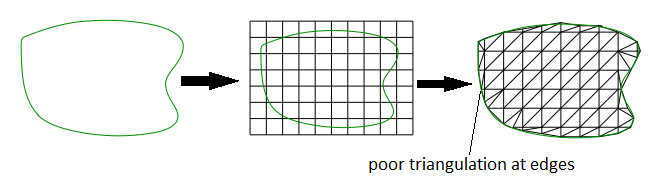
\includegraphics[scale=0.6]{figures/grid-based-triangulation.png}
	\caption{Grid-Based Triangulation}
	\label{fig:grid-based-triangulation}
\end{figure}

\subsubsection{Algorithm Summary}

\begin{table}[H]
	\centering
	\begin{tabular}{|p{4cm}|p{4cm}|p{4cm}|p{4cm}|}
		\hline	
		\textbf{Name} & \textbf{Input} & \textbf{Idea} & \textbf{Advantages/Disadvantages} \\
		\hline
		Edge Swapping & Existing triangulated mesh $T$ & Swap edge of two triangles if a different edges results in a better triangulation (by mesh quality measure $Q_1$) & Fast to do, but can cause issues as swapping an edge may result in more illegal edges (so the algorithm can sometimes take a very long time). \\
		Voronoi Tesselation & Set of points $P$ & Construct triangulation such that circumcentre of each triangle only touches the three vertices (from $P$) that belong to that triangle & Produces non-crossing triangulations of roughly even size. Quality of triangulation depends on quality of manually specified points (if points are poorly chosen, triangulation will always be poor). \\
		Delaunay Triangulation & Voronoi diagram or set of points $P$ & "" & "" \\
		Point Intersection & Existing Delaunay trinagulation $DT$  & Improve existing Delauney-style triangulation by selecting poor triangles and breaking them down in three more triangles. Process repeated until the mesh is "good enough" based on some quality measure & Good for steadily improving triangulation from a rough initial one. Can leave algorithm as long as necessary. \\
		Advancing Front Method & Set of nodes $V$ and edges $E$ which define an initial boundary ($d(v) \leq 2 \;\;\; \forall v \in V$) & Slowly construct triangles \textbf{and vertices} of the mesh by slowly advancing from a pre-defined boundary & Doesn't require user to specify the internal points of the mesh, giving the algorithm more freedom to construct good triangulations (could even have tweakable granularity/level of detail for all or parts of the mesh). \\
		Grid-Based Triangulation & Discrete or continuous boundary & Overlay a geometric shape with a grid, triangulate the grid and then alter the boundary of the grid until it matches the boundary of the given geometric shape. & Results in poor triangulation at boundaries, but very to execute. \\
		\hline		
	\end{tabular}
	\caption{Summary of Unstructured Mesh Generation Algorithms (all output triangulated meshes)}
\end{table}

\subsection{Mesh Partitioning}
\label{sec:mesh-partitioning}

After constructing a mesh which represents the situation to model the mesh needs to be partitioned so that it can be solved in \textbf{parallel by multiple processes}. This section lists techniques for partitioning arbitrary meshes across multiple processors.

\subsubsection{Good Partition Properties}

Even for structured meshes, alternative partitioning strategies exist, each of which having different speed, efficiency and scalability. A \textbf{good partition} has two main properties:
\begin{enumerate}
	\item \textbf{Equal numbers of nodes per processor} -- this provides equal load balance, so there is no idle time on any processor as they wait for other processors to finish
	\item \textbf{Minimal communication between processors} -- less communication means less overhead and a higher \textbf{efficiency factor}
\end{enumerate}
Both \textbf{block and strip partitioning} balance the load for structure meshes, but block partitioning has lower communication overheads.

These two partitioning strategies cannot be used out of the box for unstructured meshes however, and a naive random results in too much communication between processes. Consider Figure \ref{fig:unstructured-mesh-partition-example}, which shows how randomly allocating nodes/triangles results in processes containing too many nodes on process boundaries (communication required). If a more advanced strategy is used, there can be \textbf{significantly less communications overhead} and \textbf{equal load between all processors}.

\begin{figure}
	\centering
	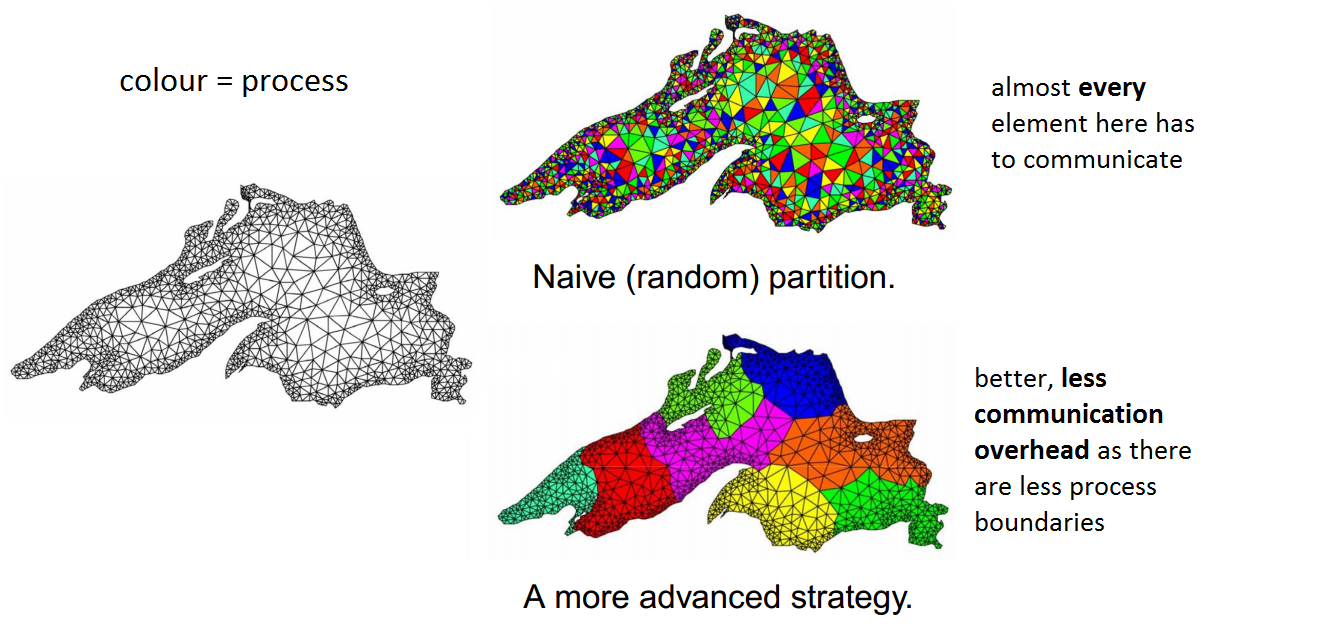
\includegraphics[scale=0.3]{figures/lake-superior.png}
	\caption{Illustration of good and bad partitioning of a non-trivial mesh (mesh based on Lake Superior)}
	\label{fig:lake-superior}
\end{figure}

Here, meshes will be considered \textbf{graphs}. Given $p$ processes, the goal is to divide the graph into $p$ \textbf{sub-graphs of equal size}, in order to provide equal load balance. The edges passing from one sub-graph to another should be \textbf{minimised}. The \textbf{cut-weight} $W$ of a partition is the \textbf{number of edges connecting different partitions} andi s used to estimate the communication costs.

TODO: figure from slides that I made showing example of cut-weights

\subsubsection{Recursive Coordinate Bisection (RBC)}

This algorithm partitions a mesh based on the \textbf{geometric location} of nodes. It has the following steps:
\begin{enumerate}
	\item Identify coordinate axis (e.g. X, Y, Z) with the \textbf{largest geometric distance} between extreme nodes (highest \textbf{range}).
	\item Choose a cut direction \textbf{perpendicular} to current exist, call this $d$
	\item Sort nodes in ascending order based on node's position on \textbf{chosen coordinate axis}
	\item Find the median node(s) of this sorted list, call it $m$
	\item Divide nodes into \textbf{two partitions} as close in size as possible. This means one partition has all the nodes left of $m$ and the other has all the nodes right of $m$ ($m$ goes in whichever makes the sizes more even)
	\item Repeat from \textbf{step 1} on \textbf{each sub-graph} until the number of partitions matches the number of processors $p$
\end{enumerate}

TODO: example from slides, referencing and following steps given above

The example in Figure \ref{fig:rcb-example} is an example of partitioning a mesh into 4 sub-graphs. It performs the following stages:
\begin{enumerate}
	\item Coordinate axis with largest range is the $x$-axis, so the first cut is perpendicular to the $x$-axis. The cut is placed at the median of the nodes sorted at the X axis (so half nodes are on the left and half are on the right). It is labelled (a) on the diagram and has a cut-eight of 5.
	\item The next cut is on the left sub-graph. The $y$-axis is the axis with the longest range and once again the cut is placed at the median of the sorted nodes. It is labelled (b) on the diagram and has a cut-eight of 4.
	\item Finally, the next cut is on the right-subgraph. The $x$-axis is the axis with the longest range, so the cut is placed at the median of the nodes sorted by their $x$ value. It is labelled (c) on the diagram and has a cut-eight of 3.
\end{enumerate}
The \textbf{total cut-weight} for this partition is $5 + 4 + 3 = 12$, as there are three cuts which cut through 5, 4 and 3 edges respectively.

\subsubsection{Recursive Graph Bisection (RGB)}

Unlike RCB, \textbf{Recursive Graph Bisection (RGB)} ignores the geometric positions of the nodes and looks more at the graph properties. Distance is the \textbf{number of edges between nodes} here, not geometric distance. Its steps are:
\begin{enumerate}
	\item Find two extreme nodes $u,v$ with are the further apart in terms of edges (have the \textbf{maximum number of edges between them})
	\item Choose one of these nodes, call it $u'$ and sort the remaining nodes in \textbf{ascending order of graph distance} from $u'$
	\item Find the median node(s) of this sorted list, call it $m$
	\item Divide nodes into \textbf{two partitions} as close in size as possible. This means one partition has all the nodes left of $m$ and the other has all the nodes right of $m$ ($m$ goes in whichever makes the sizes more even)
	\item Repeat from \textbf{step 1} on \textbf{each sub-graph} until the number of partitions matches the number of processors $p$
\end{enumerate}

TODO: example from slides, using annotiations I've addded to slides

Figure \ref{fig:rgb-example} illustrates RGB applied to the same example graph as RCB, Notice how here, the total cut-weight is 17, and not 12. RCB has produced a better partition in this case. This is not always the case, however, as the example graph in Figure \ref{fig:rcb-rgb-example-graph} shows.

Suppose we knew the cost of the \textbf{work associated with each node} and the cost of nodes $u$ and $v$ \textbf{communicating} (that is, the cost of communicating depends on the two processes). We could add those costs as \textbf{vertex edge weights} on the graph. RGB could still be used, but instead of trying to get an equal number of nodes on each process and minimising the number of cut edges, the focus becomes:
\begin{enumerate}
	\item making the total computation cost on each process as \textbf{even as possible}
	\item \textbf{minimising} the total cut-weight, which is the sum of the weights of all edges on each cut
\end{enumerate}

TODO: example from the slides with annotations

TODO: inter-processor graph!

\subsubsection{Multilevel Partitioning}

Let $G = (V, E)$ be a graph. \textbf{Graph coarsening} is when you make the graph smaller, making it a more higher-level, abstract view of the situation. A graph is coarsened like so:
\begin{enumerate}
	\item find a maximal matching $M \subseteq E$ in $G$
	\item for each edge $e = uv \in M$, merge vertices $u$ and $v$ into a single vertex $w$. All of $u$ and $v$'s neighbours are now neighbours of $w$
\end{enumerate}

TODO: basic graph coarseing example

\textbf{Multilevel Partitioning} is a more sophisticated partitioning method for a weighted graph $G$. Steps:
\begin{enumerate}
	\item Repeatedly \textbf{coarsen} the mesh to a specified level (e.g. 5 times) \textbf{retaining communication costs} (keeping totals of costs of nodes' edges in one shrunk node to nodes in another shrunk node)
	\item Carry out some partitioning algorithm on the much smaller, coarser mesh
	\item \textbf{Prolongate/extend} the partition repeatedly to the \textbf{finer meshes}, until the original mesh is reached
\end{enumerate}

Figure \ref{fig:multilevel-partitioning-idea} illustrates how you go from a large, fine graph to a small, coarse one which is then partitioned and expanded back into the original graph. Figure \ref{fig:multilevel-partitioning-example} shows an example of multilevel partitioning in action.

\begin{figure}
	\centering
	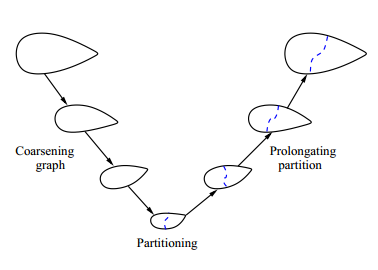
\includegraphics[scale=0.8]{figures/multilevel-partioning.png}
	\caption{Multilevel Partitioning Idea}
	\label{fig:multilevel-partitioning-idea}
\end{figure}

\begin{figure}
	\centering
	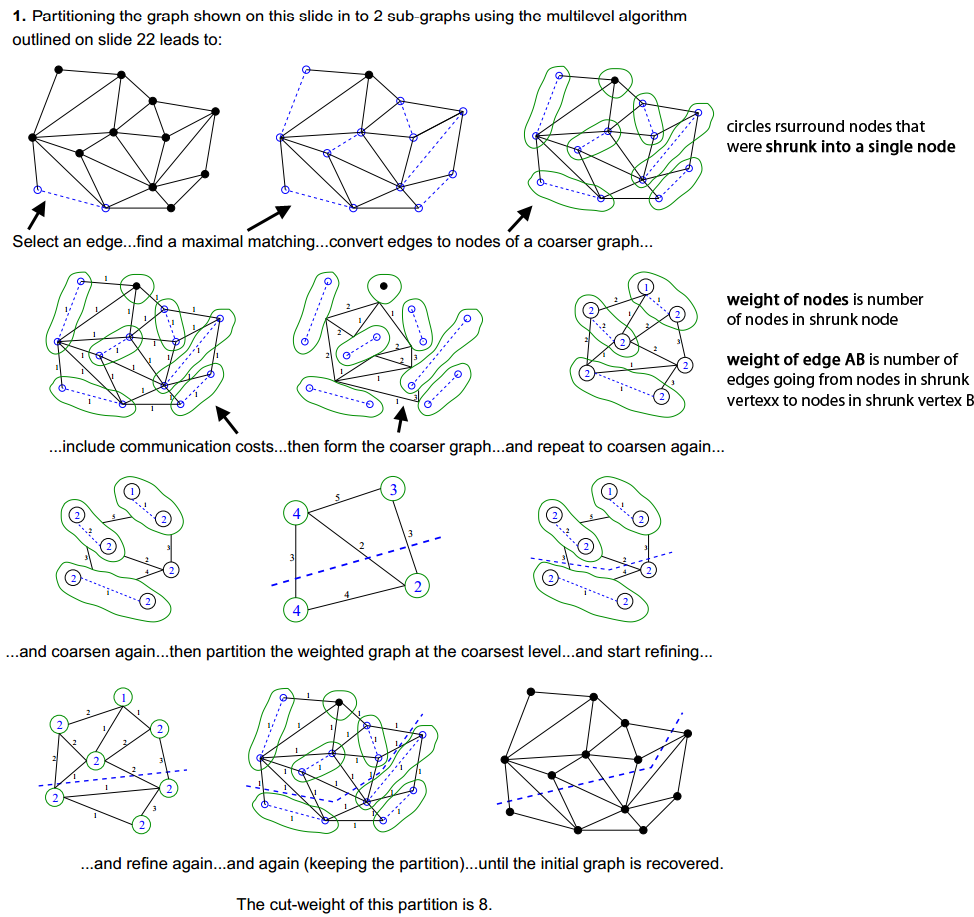
\includegraphics[scale=0.5]{figures/multilevel-partitioning-example.png}
	\caption{Example of using Multilevel Partitioning to partition a graph.}
	\label{fig:multilevel-partitioning-example}
\end{figure}

\subsubsection{Mesh Partitioning Algorithm Summary}

\begin{table}[H]
	\centering
	\begin{tabular}{|p{4.5cm}|p{6cm}|p{5.5cm}|}
		\hline	
		\textbf{Name} & \textbf{Idea} & \textbf{Advantages/Disadvantages} \\
		\hline
		Recursive Coordinate Bisection (RCB) & Find axis with largest range of values and split graph into two sub-graphs using a cut perpendicular to the found axis, such that the number of nodes on either side the cut is roughly equal. Repeat recursively for sub-graphs. & After the first cut, RCB can be done in \textbf{parallel}, with each sub-graph being sent off to another process. RCB does not take \textbf{how many edges will be cut} when deciding where to cut, which causes problems if the mesh is \textbf{non-uniform}. See Figure \ref{fig:rcb-issue} \\
		Recursive Graph Bisection (RGB) &  Find two nodes that are further apart from each other by edge distance/total edge weight. Pick one of those nodes and sort all other nodes by their distances to chosen node. find median and use that as the cut to get roughly the same number of nodes on each sub-graph. Repeat recursively for sub-graphs. & Robust to issues caused by non-uniform meshes, unlike RCB. Because RGB considers the graph form of the mesh (and not the geometric), the algorithm can still be used to find a partition with equal load and minimised communication costs, even if each node has a different amount of work and communication overhead to different nodes (they become vertex and edge weights on the graph). \\
		Multi-level Partitioning & Repeatedly simplify/coarsen graph, apply partition algorithm to smaller graph and then repeatedly expand smaller graph back to the larger, original one, maintaining the original partition. & Good for very large graphs, as finding a partition using the normal algorithms may take a very long time. Complex to implement. \\
		\hline		
	\end{tabular}
	\caption{Summary of Unstructured Mesh Partitioning Algorithms}
\end{table}

\begin{figure}
	\centering
	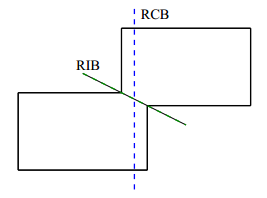
\includegraphics[scale=0.8]{figures/rcb-issue.png}
	\caption{RCB has issues with certain types of meshes, particularly unstructured ones.}
	\label{fig:rcb-issue}
\end{figure}

\subsection{Mesh Loading}
\label{sec:mesh-loading}

LECTURE 14

TODO: list of how you load meshes in and all that other stuff and eventually solve
TODO: mention some of the algorithm strategies and how you load/represent the mesh in memory in code??
TODO: even have this section???

\subsection{Adaptive Meshes}
\label{sec:adaptive-meshes}

A mesh should have enough points in all parts of the domain to accurately represent the solution of a differential equation. As more mesh points are added, the approximation should become more accurate and converge towards the correct solution. However, too many points means that the computation of the solution may take too long. It is possible to \textbf{refine} a mesh by adding more points to achieve greater accuracy in the solution.

\textbf{Uniform mesh refinement} is when greater detail is added to all parts of the mesh, uniformly. That is, the same amount of new points is added every. Consider the heat diffusion problem. Refining the mesh for this to include more points gives more much \textbf{smoother, detailed} approximations, as Figure \ref{fig:uniform-refinement} shows.

Doing more work gives better approximations, but we need to decide when the approximation is "good enough". It is best to assess where doing the extra would be \textbf{most beneficial} and refine the mesh there. Uniformly refining an entire mesh adds many more nodes and is very expensive, both in terms of memory and CPU time. Often, the fine resolution is \textbf{only needed in certain regions} (not entire mesh), so those regions of interest are refined. This is known as \textbf{adaptive meshes/local mesh refinement}.
 
Using adaptive meshes allows the desired level of accuracy to be obtained with \textbf{less work and memory}. However, some of the simplicity of structured meshes is lost when are refined adaptively. Figure \ref{fig:local-refinement-structured-mesh} shows a structured mesh being refined in a specific region, producing a \textbf{non-uniform} structured mesh. Not only has this \textbf{lost some of the simplicity} that made structured meshes easier to implement and compute (e.g. uniform grid structure where indices tell you what nodes are adjacent), but it also \textbf{added work that wasn't desired}. To add detail to the centre of the mesh has mean more points have had to be added elsewhere, so the structure is retained.

\begin{figure}
	\centering
	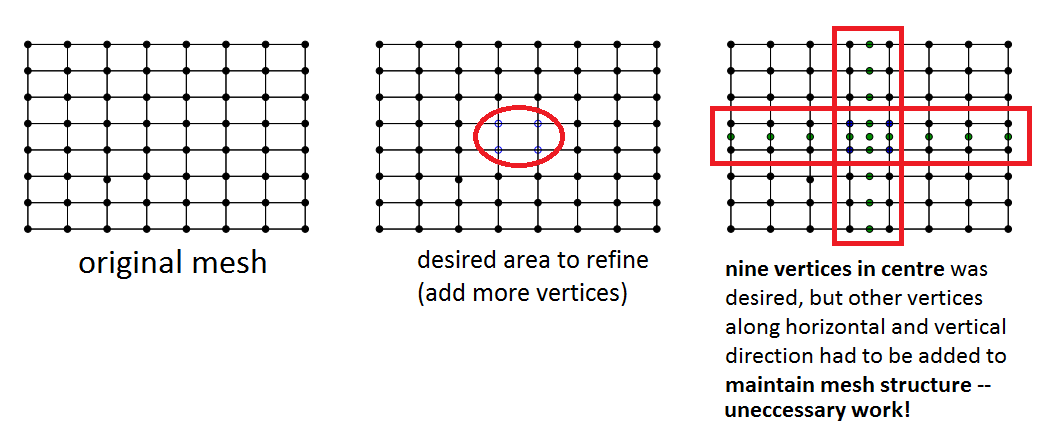
\includegraphics[scale=0.5]{figures/uniform-mesh-refinement.png}
	\caption{Refining uniform meshes often leads to unnecessary work as extra vertices are added to places where they aren't needed to maintain a mesh's structure}
	\label{fig:local-refinement-structured-mesh}
\end{figure}

Unstructured meshes should be refined in such a way that the mesh quality measure is preserved. Additionally, refinement makes it even more \textbf{complicated} to implement solvers in parallel, especially if the mesh is refined/evolved as the simulation is running.

\subsubsection{Local Error Estimation}

The results of a simulation can be used to provide an estimate on \textbf{where the most significant errors} introduced by the computational model are. From this, you can selectively increase resolution where it will have the most effect (at the regions with high error). This knowledge can be used to guide improvement of the mesh, the discretisation and/or the solution algorithm. This method of looking at the solution obtained, using it to find areas of maximum error and refining those areas is known as a \textbf{posteriori error estimation}.

\subsubsection{Refining Triangular Meshes}

Many unstructured meshes are triangular meshes, so how to we define a triangular mesh? Figure \ref{fig:isolated-triangle-refinement} shows how an \textbf{isolated triangle} can be refined. You:
\begin{enumerate}
	\item place a new node at the midpoint of \textbf{edge edge}
	\item form \textbf{sub-triangles} by joining these nodes
\end{enumerate}
This is similar to how you would split a square into four squares.

\begin{figure}
	\centering
	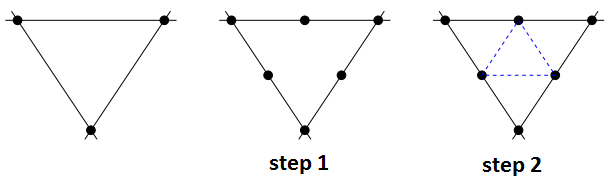
\includegraphics[scale=0.6]{figures/single-mesh-triangulation.png}
	\caption{Refining an isolated triangle}
	\label{fig:isolated-triangle-refinement}
\end{figure}

Refining a whole triangular mesh requires all little more care, however. Refining single triangles creates \textbf{hanging nodes} (see Section \ref{sec:structured-unstructured-problems}) in the overall mesh. \textbf{Red-green refinement} deals with hanging nodes, but then extra care needs to be made to ensure \textbf{mesh quality} is preserved. Figure \ref{fig:red-green-refinement} shows a detailed example of red-green refinement. The key take-out is that running such a procedure results in a refined mesh which:
\begin{itemize}
	\item has no hanging nodes
	\item has no adjoining "green" triangles
	\item has required a lot of bookkeeping to construct, meaning such a procedure is difficult to implement and expensive to compute
\end{itemize}

TODO: figure showing overall process of refining mesh

There are three standard approaches to improving the accuracy of the approximation by refining the mesh:
\begin{itemize}
	\item \textbf{$\mathbf{h}$-refinement} -- adds more nodes to reduce element length $h$
	\item \textbf{$\mathbf{r}$-refinement} -- moves the positions of the nodes. One advantage to this is that it has no affect on the partitioning of the problem for parallel computation, as no nodes/edges are created/destroyed.
	\item \textbf{$\mathbf{p}$-refinement} -- increases the order of the polynomial approximation ($y = x^p + ...$) between the nodes. Results in more accurate representation of what's going on between the nodes, instead of just the \textbf{linear central differences}
\end{itemize}

\subsubsection{Mesh Adaptivity in Parallel Simulations and Dynamic Load Balancing}

Local adaptivity can be used in \textbf{parallel} simulations too. The sub-graph/mesh a processor has could be adapted locally, without the neighbouring processes \textit{even knowing}. However, care is needed with the communication of data across \textbf{processor boundaries}.

When local adaptation is carried out in a parallel computation, the work per processor change. This means \textbf{load balance}, which results in idle time and a reduction in the \textbf{efficiency factor}. The communication pattern may also change, further reducing efficiency. As a mesh is refined on a processor, any static load balancing achieved by the initial partition is \textbf{no longer valid}, so dynamic loading balancing must be used.

There are two forms of dynamic loading balancing:
\begin{itemize}
	\item \textbf{Repartitioning} -- this performs a new static load balance by fully partitioning the adapted mesh. This is very expensive to perform, and doesn't guarantee that the right data will be retained in the right processors, meaning that a restart of the simulation may be required. 
	\item \textbf{Data Migration} -- this adjusts the current partition by shifting data between neighbouring processors. This requires a way to determine what data to move, how much of it and where to move it to.
\end{itemize}

Both these are very expensive and often \textbf{dominate} the time it takes to actually solve the system of equations itself, as shown by Table \ref{tab:dynamic-load-balancing-costs}. There are costs associated with the imbalance in load that occurs when the mesh is adapted, calculating a new partition and transferring data to new processors. All of this adds up, so the decision to use dynamic load balancing must be made carefully.

\begin{table}
	\centering
	\begin{tabular}{|l|l|}
		\hline
		\textbf{Operation} & \textbf{Time} \\
		\hline
		Repartition time & 3.0 - 15.2s \\
		Migration time & 17.8 - 37.8s \\
		Solve time & 2.54 - 3.11s \\
		\hline
	\end{tabular}
	\caption{$10^6$ mesh elements with adaptive refinement on an SGI Origin 2000}
	\label{tab:dynamic-load-balancing-costs}
\end{table}

\subsubsection{Diffusion Method}

The \textbf{Diffusion Method} is an approach to data migration based on physical diffusion. Each processor exchanges some of its load with neighbouring processes, with the amount exchanged proportional to the differences in the loads.

Let $G = (V, E)$ be a \textbf{subdomain graph}, in which the nodes represent processors and the edges represent links between them (processor boundaries). The steps of the algorithm are as follows:
\begin{enumerate}
	\item Assign each processor/vertex $i \in V$ a number $l_i$ representing the load on processor $i$.
	 \item For each processor $i \in V$, iterate as follows:
	 \begin{enumerate}
	 	\item for each node $j \in V$ connected to $i$:
	 		\begin{enumerate}
	 			\item calculate the \textbf{load difference} between $i$ and $j$, $d_{ij} = (l_i^{(k)} - l_j^{(k)})$
	 			\item calculate the coefficient $c_{ij} = \frac{1}{\max (degree(i), degree(j)) + 1}$
	 		\end{enumerate}	 		
	 	\item update total load on vertex $i$ after exchanges with $l_i^{(k+1)} = l_i^{(k)} - \sum_j {c_{ij}d_{ij}}$
	 \end{enumerate}
\end{enumerate}
This algorithm \textbf{always converges} for connected graphs and is at worst $O(p^2)$ if integer values are used.

Consider the partition of a mesh into four regions on the left of Figure \ref{fig:diffusion-method-example} which, after local adaptive mesh refinement, has the processor loads indicating in the graph on the right.

Let's do an iteration of the algorithm. First, we compute $c_{ij}$ for $i \in \lbrace 1, 2, 3, 4 \rbrace$. This results in:
\begin{equation}
	c_{12} = c_{13} = c_{14} = c_{23} = c_{34} = \frac{1}{4}
\end{equation}
Now we compute the load differences $d_{ij}$ :
\begin{multline} \\
	d_{12} = (439 - 443) = -4 \;\;\;\;\;\;\;\; d_{13} = (439 - 441) = -2 \\
	d_{14} = (465 - 439) = -26 \;\;\;\;\; d_{23} = (443 - 441) = 2 \\
	d_{34} = (441 - 465) = -24 \\
\end{multline}
Multiplying the two values together and \textbf{rounding to the largest integer in terms of magnitude}, gives us:
\begin{multline} \\
	1 \iff 2 \; : \;\;\;\;\; c_{12}d_{12} = \frac{1}{4}(-4) = -1 \\
	1 \iff 3 \; : \;\;\;\;\; c_{13}d_{13} = \frac{1}{4}(-2) = -1 \\
	1 \iff 4 \; : \;\;\;\;\; c_{14}d_{14} = \frac{1}{4}(-26) = -7 \\
	2 \iff 3 \; : \;\;\;\;\; c_{23}d_{23} = \frac{1}{4}(2) = 1 \\
	3 \iff 4 \; : \;\;\;\;\; c_{34}d_{34} = \frac{1}{4}(-24) = -5 \\
\end{multline}
This means that one "work item" will be moved from node 2 to 1 (-1 for $1 \iff 2$), one will be moved from node 3 to 1, seven will be moved from node 4 to 1, 1 will be moved from node 2 to 3 and 5 will be moved from 4 to 3.

Figure \ref{fig:diffussion-method-example2} shows iteration one in action, with the first graph being the work moving to/from node 1, the second graph being the work moving to/from nodes 2 and 3 and the final graph being the work on each process after the iteration. Figure \ref{fig:diffussion-method-example3} shows another two iterations, at which point the algorithm \textbf{terminates} because it has converged to an equal load balance.

\begin{figure}[H]
	\centering
	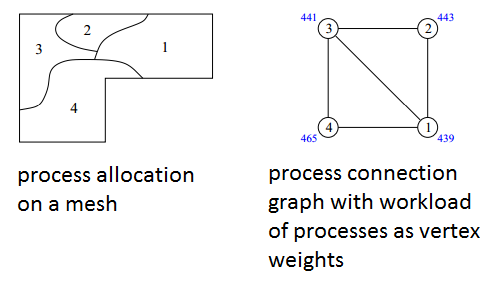
\includegraphics[scale=0.5]{figures/diffusion-method-example1.png}
	\caption{Mesh with existing partition across four processes}
	\label{fig:diffussion-method-example}
\end{figure}

\begin{figure}[H]
	\centering
	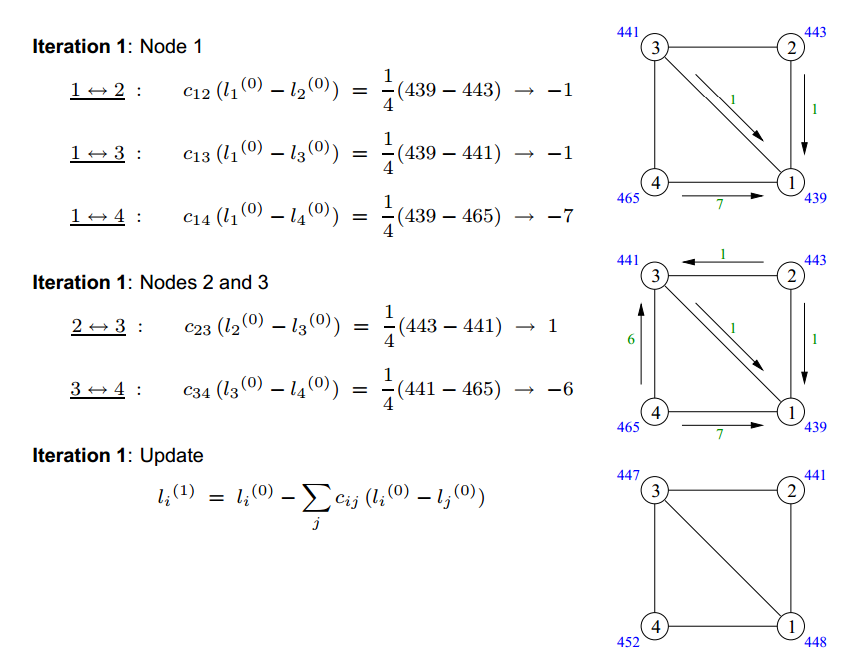
\includegraphics[scale=0.5]{figures/diffusion-method-example2.png}
	\caption{Iteration 1 of diffusion method}
	\label{fig:diffussion-method-example2}
\end{figure}

\begin{figure}[H]
	\centering
	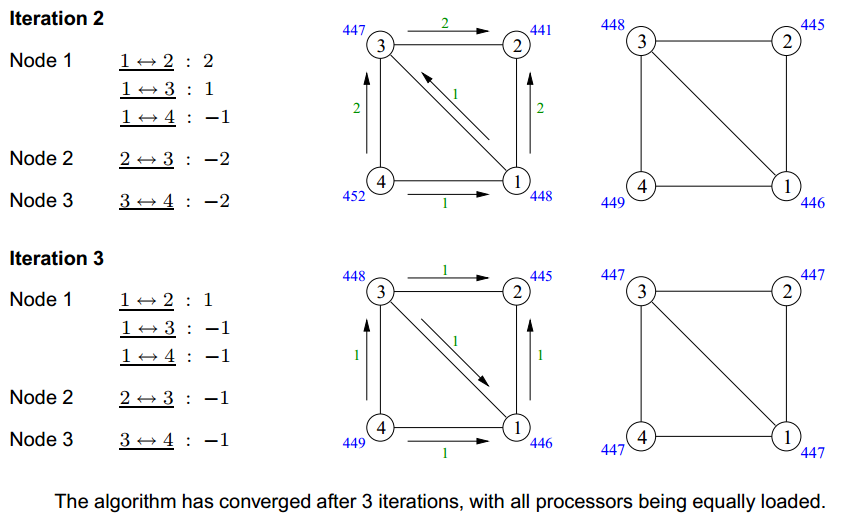
\includegraphics[scale=0.5]{figures/diffusion-method-example3.png}
	\caption{Iterations 2 and 3 of diffusion method, showing convergence}
	\label{fig:diffussion-method-example3}
\end{figure}

\section{MPI}

\subsection{Overview of MPI Paradigm}

The most common mechanism for transferring data between processes with their own distributed memory is to pass a message between these processes. MPI (Message-Passing Interface) is a definition of a message passing library and is widely used for parallel computing. It allows communication of data between distributed memory processes and has standard libraries for C, C++ and FORTRAN. It is very low level however, meaning each individual communication must be programmed by hand.

Two primary mechanisms are required to execute MPI programs:
\begin{enumerate}
	\item a method of creating separate processes on different computers (remotely)
	\item a method of sending and receiving messages
\end{enumerate}
For the first step, the command \texttt{mpiexec} can be used to start a fixed number of processes on any number of machines specified. Each process runs the same program (SPMD), allocating memory and doing computations until the parallel portion of the code starts. This start is marked by:
\begin{lstlisting}[language=C,frame=single]
int noprocs;
int nid;
MPI\_Init(&argc, &argv);
MPI\_Comm\_size(MPI_COMM_WORLD, &noprocs);
MPI\_Comm\_rank(MPI_COMM_WORLD, &nid);
\end{lstlisting}

After this point, the parallel portion has begun and each process knows where it fits in the system (what it's ID, or rank, is). The parallel code continues until \texttt{MPI\_Finalize()} is called, at which point all the programs become independent programs again. Note that only one process should handle I/O -- this is typically the master process. The skeleton for an MPI C program is given in the listing below.

MPI follow the SPMD model, where programs execute the same code. However, most situations do require one or more processes to execute different code. To do this, if-statements checking the rank of current process can be inserted the code to give processes different behaviour. A master-worker structure can be implemented by \textbf{checking if a process has ID/rank 0} -- if it does, then it's the master and performs the master logic.

The listing below is the skeleton of a C MPI program, which also implements a check to see if the current process is the master process.
\begin{lstlisting}[language=C,frame=single]
#include <stdio.h>
#include <mpi.h>
int main(int argc, char** argv)
{
	int noprocs, nid;
	MPI\_Init( &argc, &argv );
	MPI\_Comm\_size( MPI\_COMM\_WORLD, &noprocs );
	MPI\_Comm\_rank( MPI\_COMM\_WORLD, &nid );
	
	if (nid == 0)
		master();
	else
		worker();	
	
	MPI\_Finalize();
	return 0;
}
\end{lstlisting}

\subsection{Sending and Receiving Messages}

\paragraph{Syntax for sending messages:}
\texttt{int MPI\_Send(void *buf, int count, MPI\_Datatype datatype, int dest, int tag, MPI\_Comm comm)}

\textbf{Input Parameters:}
\begin{itemize}
	\item \textbf{buf} -- initial address of send buffer (choice)
	\item \textbf{count} -- number of elements in send buffer (nonnegative integer)
	\item \textbf{datatype} -- datatype of each send buffer element (handle)
	\item \textbf{dest} -- rank of destination (integer)
	\item \textbf{tag} -- message tag (integer)
	\item \textbf{comm} -- communicator (handle)
\end{itemize}

\paragraph{Syntax for receiving messages:}
\texttt{int MPI\_Send(void *buf, int count, MPI\_Datatype datatype, int dest, int tag, MPI\_Comm comm)}

\textbf{Output Parameters:}
\begin{itemize}
	\item \textbf{buf} -- initial address of receive buffer (choice)
	\item \textbf{status} -- status object (Status)
\end{itemize}
\textbf{Input Parameters:}
\begin{itemize}
	\item \textbf{count} -- maximum number of elements in receive buffer (integer)
	\item \textbf{datatype} -- datatype of each receive buffer element (handle)
	\item \textbf{source} -- rank of source (integer)
	\item \textbf{tag} -- message tag (integer)
	\item \textbf{comm} -- communicator (handle)
\end{itemize}

\subsection{Synchronous and Asynchronous}

\textbf{Synchronous Message Passing} is when a process \textbf{blocks} until the message has fully been sent or received. The two functions described in the previous section are examples of synchronous message passing -- they only return when the message transfer is complete. This blocking mechanism synchronises the communication process.

However, this synchronisation mechanism introduces overhead and can slow the code down, often unnecessarily (e.g. a process could compute something else while waiting for some data from another process). It is possible to send messages where the functions \textit{do not wait} for the message transfer to complete before retuning. This is known as \textbf{asynchronous message passing}. With this mechanism, processes can move forward sooner, as long as due is taken. There are no kinds of asynchronous communication -- locally blocking and non-blocking.

\textbf{Locally blocking} communication means that data is stored in a separate buffer and then sent to the target process. This is done so that the send function can return before it's actually been received by the target process, but means it's safe to write to the memory area that was sent. This is because the data to send has been copied to a local buffer before being sent (as illustrated in Figure \ref{fig:local-comm-buffer})

TODO: local comm buffer diagram

\paragraph{\textbf{NOTE:}} Locally blocking receive operations simply wait until the message as been received, similar to completely synchronous receives.

\textbf{Non-blocking communication} means that the send and receive functions return \textit{immediately}, even if the data has been successfully sent from, or received to, the local buffer. This is shown in Figure \ref{fig:non-block-comm}. Therefore, the local buffer may not even be safe to read as it may not have the correct data in. Additionally, it is not safe to write to since the process be overwriting data that hasn't actually been sent to the other process yet. Therefore, it is up to the programmer to ensure that this isn't a problem!

TODO: non-blocking send diagram

Finally, greater synchronisation can be achieved by explicitly checking for the completion of a particular operation, using the following functions:
\paragraph{ \texttt{MPI\_Wait(request, status)}} -- \textbf{blocks} until the operation indicated by \texttt{request} is completed before returning control
\paragraph{ \texttt{MPI\_Test(request, flag, status)}} -- \texttt{returns immediately} with boolean value \texttt{flag} indicating whether the operation indicated by \texttt{request} has completed

Manually waiting offers greater flexibility as it allows you to choose when to block. This means you could receive a message, perform some computation  while waiting for it be received and then after that computation is done and the data being received is required, wait/block until it has been received.

\paragraph{\textbf{NOTE}:} With any kind of synchronisation, you still have the possibility of \textbf{DEADLOCK}.

\subsection{Global Communication}

The previous methods of communication covered is known as \textbf{point-to-point communication}, which is when a single source transmits data to a single destination. It is possible for a single process to broadcast data to a multiple processes, or multiple processes send their data to the same process, which aggregates them in some form. This sections describe some of these \textbf{global communication} methods.

\subsubsection{One-to-Many}

The same message can be broadcast to \textit{all} of the process using:
\texttt{MPI\_BCast(buf, count, datatype, root, comm);}
where \textit{root} is the rank of the root process which is performing the broadcast. This exact same command should be executed by all the processes; the root process uses it to \textit{send} the data and all the other processes use it to block and \textit{receive} the data.

A root process can also \textbf{scatter} its contents so specific parts are send to different processes. This could be used to distribute elements of an array for example. The command is below:

\paragraph{} \texttt{MPI\_Scatter(sendbuf, sendcount, sendtype, recvbuf, recvcount, recvtype, root, comm)}

\subsubsection{Many-to-One}

The reverse of the scatter operation is the \textbf{gather} common. Here, a single process gathers messages from different processes into a single long array.

\paragraph{} \texttt{MPI\_Gather(sendbuf, sendcount, sendtype, recvbuf, recvcount, recvtype, root, comm)}
\paragraph{}

When gathering multiple messages, it is often required to carry out arithmetic or logical operations on the numerical messages returned from the other processes. This is possible with the \textbf{reduce} command:

\paragraph{} \texttt{MPI\_Reduce(sendbuf, recvbuf, count, recvtype, op, root, comm)}
\paragraph{}

This command performs the same operation on all of the data items returned and stores the aggregate result in a single value. \texttt{op} is the operation to perform; example values include \texttt{MPI\_MAX}, \texttt{MPI\_MIN}, \texttt{MPI\_SUM} and \texttt{MPI\_PROD}.		

\subsubsection{Many-to-Many}

Sending messages from all processes to all other processes can done using:

\paragraph{} \texttt{MPI\_Alltoall(sendbuf, sendcount, sendtype, recvbuf, recvcount, recvtype, root, comm)}

However, it can be difficult matching the send and receive buffers exactly, as a lot of data is being to and from this single command.

\subsection{Load Balancing}

It is ideal to distribute the work \textbf{evenly} between processes, as this prevents some processes being overworked and running slowly and others from waiting around for more work. The process of trying to distributing work evenly is known as \textbf{load balancing}.

\textbf{Embarrassingly parallel} problems refer to problems where computation can obviously be divided into a number of completely \textbf{independent} parts (e.g. matrix sum). This means that each part can be executed on a separate process without requiring extra communication. Load balancing with these problems is easy. Examples of embarrassingly parallel problems include:
\begin{itemize}
	\item vector dot/scalar product
	\item matrix sum
\end{itemize}

For others problems however, it is not obvious how work can be divided evenly, especially when you want each process to be completely independent so no extra communication is required.

\textbf{Static load balancing} is used when work can be allocated at the start of the computation, with each processor having a fixed task to perform (defined at the start). This can be used if you \textbf{know the size} of the problem beforehand (such as summing/multiplying matrices).

\textbf{Dynamic load balancing} is used when the optimal division of work depends on \textbf{specific problem parameters} which alter the amount of computation required per chunk of the problem. When it's not known how much computation is going to be required in advance, it is not possible to distribute the work evenly at the start of computation. Dynamic load balancing allocates work throughout the entire computation process.

An example of a problem in which you don't the computation in advance is for generating an image of the \textbf{Mandelbrot set}. Some pixels require more computation (recursion) than others, so if you just farm the rows of the image to different processes, the work is still is not split evenly since some collections of rows may take more computation than others. This means there'll be many processes waiting for the processes which have more work to finish (waste of resources).

\textbf{Work Farms} (or pools) are a simple way of dynamically balancing work load across multiple processes. It has the following steps:
\begin{enumerate}
	\item divide problem into many work packages, many more than the number of processes
	\item send each processes one work package to carry out
	\item as soon as a processor has completed its work and notified the root processor, send it a new work package
	\item repeat step 3 until all work packages are complete
\end{enumerate}

This will cause faster processors (or processes that happen to get smaller work packages) to get more work to keep them busy, resulting in less waiting time. This not only handles the case where work is difficult to distribute evenly in advance, but it also handles the case where some process are simply faster than others (better hardware, smaller communication times, etc.).

Applying work farms to the Mandelbrot set example, the rows of the image could be work packages. Processes which receive "easy" rows of the image will complete faster, but it does not matter since those processes will just get more work to complete while other processes are still dealing with "harder" rows.

\subsection{MPI Usage}

Common MPI tasks:
\begin{tabular}{lp{10cm}}
	\textbf{Build MPI Program} & \texttt{mpicc -Wall -o <execName> <sourceFiles>} \\
	\textbf{Start MPD Ring} & \texttt{mpdboot --file=<machineSpecFilename> -n <numMachines> --ncpus=<numCPUsPerMachine>} \\
	\textbf{Stop MPD Ring} & \texttt{mpdexitall} \\
	\textbf{See Current MPD Jobs} & \texttt{mpdallexit} \\
	\textbf{Execute MPI Program} & \texttt{mpi-exec -n <numProcessesToUse> <pathToExecutable>} \\
\end{tabular}

\paragraph{}

Format of machine specification file:
\begin{lstlisting}
hostname:ncpus
hostname:ncpus
hostname:ncpus
hostname:ncpus
\end{lstlisting}

\end{document}
